\documentclass{sbmlmanual}

\newcommand{\libsbml}{\textsc{libsbml}}

\begin{document}

%=============================================================================
% Title page
%=============================================================================

\title{\libsbml{}\\[5pt]
  Developer's Manual}

\author{Ben Bornstein}

\authoremail{bornstei@cds.caltech.edu}

\address{The SBML Team\\
  Control and Dynamical Systems, MC 107-81\\
  California Institute of Technology, Pasadena, CA 91125, USA\\[2pt]
  {\url{http://www.sbml.org/}}}

\date{DRAFT\\[5pt]
  \today{}\\[10pt]%
  \hspace*{-1ex}\libsbml{} Version \input{../../VERSION.txt}%
}

\maketitlepage


%=============================================================================
\section{Quick Start}
\label{sec:quickstart-unix}
%=============================================================================

\libsbml{} requires a separate XML library for low-level XML tokenizing and
Unicode support.  It currently supports the Xerces-C++ and Expat XML
libraries on Linux, Solaris, Windows and MacOS X.  You will first need to
make sure one of these libraries is installed on your system.  Many Linux
systems provide one or both of these libraries either as part of their
standard distribution or as an optional RPM or Debian package.  For more
information, see \url{http://xml.apache.org/xerces-c/} for Xerces and
\url{http://expat.sf.net} for Expat.

%-----------------------------------------------------------------------------
\subsection{Linux, Solaris, Cygwin or MacOS X}
%-----------------------------------------------------------------------------

If you have obtained the source code distribution, then at your Unix,
Cygwin or MacOS~X command prompt, unpack the distribution, \shell{cd} into
the directory created (e.g., \shell{libsbml-2.0.3/}), and type the
following command to configure \libsbml{} for your system:

\begin{example}[csh]
  ./configure
\end{example}

To specify Expat explicitly rather than the \libsbml{} default of Xerces,
use a command such as the following instead (and make sure to read about
the limitations surrounding the use of Expat explained in
Section~\ref{sec:installation}):

\begin{example}[csh]
  ./configure --with-expat
\end{example}

Next, compile and install the \libsbml{} library using the following command:

\begin{example}[csh]
  make
  make install
\end{example}

To compile programs that use libsbml with GCC (for an example, see
Section~\ref{sec:read-example}):

\begin{example}[csh]
  gcc -o myapp.c myapp.c -lsbml
\end{example}


%-----------------------------------------------------------------------------
\subsection{Windows}
%-----------------------------------------------------------------------------

Unzip the \libsbml{} distribution and open the resulting folder (which will
have a name such as \shell{libsbml-2.0.3-expat} or
\shell{libsbml-2.0.3-xerces}).  There are debug (\shell{libsbmld}) and
release (\shell{libsbml}) versions of \libsbml{}, with \shell{.dll} and
\shell{.lib} files for both versions in the \shell{win32} subdirectory of
the \libsbml{} distribution.  Header files are located in the subdirectory
\shell{src/sbml}.

Users of Visual C++ should make their Visual C++ projects link with the
files \shell{libsbml.lib} or \shell{libsbmld.lib} and generate code for the
Multithreaded DLL or Debug Multithreaded DLL version of the VC++ runtime,
respectively.


%=============================================================================
\section{Introduction}
\label{sec:introduction}
%=============================================================================

This manual describes \libsbml{}, a C application programming interface
(API) library for reading, writing and manipulating the Systems Biology
Markup Language~\citep[SBML;][]{hucka_2001b,hucka_2003,finney_2003b}.
Currently, the library supports all of SBML Level~1 Version~1 and
Version~2, and nearly all of SBML Level~2 Version~1.  (The
still-unimplemented parts of Level~2 are: support for RDF, and support for
MathML's \code{semantics}, \code{annotation} and \code{annotation-xml}
elements.  These will be implemented in the near future.)  For more
information about SBML, please see the references or visit
\url{http://www.sbml.org/} on the Internet.  \libsbml{} is entirely
open-source under the terms of the GNU LGPL, and all source code and other
materials are freely and publicly available.

Because the library provides a C API, the rest of this manual assumes
familiarity with the C programming language.  Some parts of the library
were written in C++, however, experience with C++ is not required; its use
is ``hidden'' behind C functions.  A companion
document~\citep{bornstein_2004b} provides a detailed reference manual for
the API.

Some of the technical features of \libsbml{} include:

\begin{itemize}
  
\item \textbf{\textsl{Small Memory Footprint}}:  The parser is event-based (SAX2)
  and loads SBML data into C structures that mirror the classes in the SBML
  specification.  No intermediate DOM is used, which greatly reduces
  runtime memory usage.
  
\item \textbf{\textsl{Fast Runtime}}:  A 2000 reaction test file
  (\url{http://www.gepasi.org/gep3sbml.html}) loads in 1.18s on a 1 GHz AMD
  Athlon XP and uses 1.4Mb of memory.
  
\item \textbf{\textsl{Portable}}:  The C source code is pure ISO standard C for
  maximum portability.  It produces no errors or warnings when compiled
  with either GCC or Microsoft Visual C++.  GCC compilation flags are:
  \shell{-ansi -pedantic-errors -Wall}, i.e., ISO violations are
  compilation errors instead of warnings and all warnings are reported.
  The build system uses the GNU Autotools (Autoconf, Automake, and Libtool)
  to build shared and static libraries on a variety of Unix-based
  platforms.  Microsoft Windows is supported either through the Cygwin
  environment or as a native Win32 Dynamic Link Library (DLL).  A Microsoft
  Visual C++ 6.0 project file is included in the source distribution and 
  precompiled Windows distributions are available.
  
\item \textbf{\textsl{Full SBML Support}}:  All constructs in SBML Level~1
  (Versions~1 and~2) and SBML Level~2 are supported, with the exceptions
  noted above (i.e., RDF, and three rarely-used MathML constructs).  The
  exceptions will be removed in the near future.  \libsbml{} handles such
  SBML differences as the alternate spellings of \emph{species} and
  \emph{annotation} between the SBML specifications.
  
  The full-text of \code{<notes>} and \code{<annotation>} elements (the
  latter including namespace declarations) may be retrieved from any
  SBML object.  For compatibility with some technically incorrect but
  popular Level~1 documents, the parser recognizes and stores notes
  and annotations defined for the top-level \code{<sbml>} element (logging
  a warning).
  
\item \textbf{\textsl{Full XML Schema Validation}}: The library can use the Apache
  Xerces-C++ XML library, which supports full XML Schema validation.  All
  XML and Schema warning, error and fatal error messages are logged with
  line and column number information and may be retrieved and manipulated
  pragmatically.  The XML Schema file used by the parser for validation is
  configurable.
  
\item \textbf{\textsl{Full Unicode Support}}: SBML Documents are parsed and
  manipulated in the Unicode codepage for efficiency (this is Xerces-C++
  native format); however, strings are transcoded to the local code page
  for the SBML C interface data structures.
  
\item \textbf{\textsl{Well Tested}}: The entire library was written using
  the test-first approach popularized by Kent Beck and eXtreme Programming,
  where it's one of the 12 principles.  Currently the \libsbml{} code base
  features 3340 individual assertions in 636 functional unit tests.  Four
  test cases are responsible for reading entire SBML files (three are
  examples from the SBML Level~1 specification) into memory and verifying
  every field of the resulting structures.
  
\item \textbf{\textsl{Conscientious Use of Memory}}: All memory for and contained in
  SBML structures is C memory, so \code{realloc()} and \code{free()}
  may be used.  This is an important distinction when working with mixed C
  and C++ code.  C's \code{malloc()} and \code{free()} are not
  compatible with C++'s \code{new} and \code{delete} operators.

  A custom memory trace facility can be used to track all memory
  allocated and freed in both the library and all test suites.  This
  facility must be enabled at build time with \shell{./configure
  --enable-memory-tracing}.  For performance reasons memory tracing
  should be turned off in production environments.

\end{itemize}


%=============================================================================
\section{Detailed Installation Instructions}
\label{sec:installation}
%=============================================================================

The \libsbml{} distributions can be downloaded from the \emph{SBML} project
area on SourceForge.net, at \url{http://sf.net/projects/sbml}.  A link to
the download area is also provided on the SBML project home page,
\url{http://www.sbml.org}.

\libsbml{} depends on a separate XML library for low-level XML tokenizing
and Unicode support.  Currently, \libsbml{} can use either Apache's
Xerces-C++ XML library or James Clark's Expat XML library on Linux,
Solaris, Windows and MacOS~X.  You will first need to make sure one of
these libraries is installed on your system.  Many systems provide one or
both of these libraries either as part of their standard distribution or as
an optional RPM or Debian package.  DLL and LIB file distributions are
available for both Xerces and Expat.  For more information, see the
following resources:

\begin{itemize}\setlength{\parskip}{-0.25ex}

\item Xerces: \url{http://xml.apache.org/xerces-c/}
\item Expat: \url{http://expat.sf.net}

\end{itemize}

Note that if you use Expat instead of Xerces, \libsbml{} will not be able
to perform certain kinds of validation tests on SBML models, because Expat
is not a validating XML parser.  A validating parser can check XML input
against an XML Schema.  Xerces is currently the only validating parser
library usable with \libsbml{}.  Using Expat with \libsbml{} effectively
means it will be unable to check SBML input against the SBML XML Schema.
The tradeoff is that Expat can be noticeably faster at parsing large models
than Xerces.

Unless instructed otherwise, the \libsbml{} build process will
\textbf{default to using Xerces}.  A good way to determine whether
Xerces-C++ is installed on your system is to run the configuration command
(see below); it will halt if it cannot find the Xerces-C++ library.  You
can provide the configuration command with a flag telling it to use Expat
instead of Xerces and you can indicate where the libraries are located if
they are not in standard locations on your system.

\libsbml{} is designed to be extremely portable.  It is written in 100\%
pure ISO~C and the build system uses the GNU Autotools (Autoconf, Automake
and Libtool).  

\subsection{Unpacking and Configuring \libsbml{}}

First, uncompress and unpack the \libsbml{} sources.  Then, configure the
package by typing the following command at your Unix, Cygwin or MacOS~X
command prompt:

\begin{example}[csh]
  ./configure
\end{example}

To specify Expat explicitly rather than the \libsbml{} default of Xerces,
use a command such as the following instead:

\begin{example}[csh]
  ./configure --with-expat
\end{example}

If either Expat or Xerces is installed in a non-standard location on your
computer system (e.g., a home directory), \shell{configure} will not be
able to detect it.  In this case, \shell{configure} needs to be told
explicitly where to find the libraries.  Use the following forms:

\begin{example}[csh]
  ./configure --with-expat=|\emph{dir}|
\end{example}
or
\begin{example}[csh]
  ./configure --with-xerces=|\emph{dir}|
\end{example}

where \code{\emph{dir}} is the \textbf{parent} directory of where the
\code{include} and \code{lib} directories of Xerces or Expat (whichever
one you are trying to use) is located.  For example, on MacOS~X, if you
used Fink to install Expat in Fink's default software tree, you would
configure \libsbml{} using the following:

\begin{example}[csh]
  ./configure --with-xerces=/sw
\end{example}

During the installation phase (i.e., during \shell{make install},
discussed below), the \libsbml{} installation commands will copy header
files to \shell{/usr/local/include/sbml} and (shared and static) library
files to \shell{/usr/local/lib}, by default.  To specify a different
installation location, use the \shell{--prefix} argument to
\shell{configure}.  For example,

\begin{example}[csh]
  ./configure --prefix=/my/favorite/path
\end{example}

Of course, you can combine the flags to \shell{configure}, giving both
\shell{--prefix} and \shell{--with-expat} or \shell{--with-xerces} to set
both options.  Other options are described below.


\subsection{Building and Installing \libsbml{}}

Once configured, building should be very easy.  Simply execute the
following commands at your Unix, Cygwin or MacOS~X command prompt:

\begin{example}[csh]
  make
  make install
\end{example}

If all went as it should, \libsbml{} should end up compiled and installed
on your system, in either the default location (\shell{/usr/local/}) or in
the location you indicated during the configuration step as explained
above.  And that that's all that should be required to build and install
\libsbml{} normally!


\subsection{Additional Options for Configuring \libsbml{}}

In addition to the \shell{--prefix}, \shell{--with-expat} and
\shell{--with-xerces} options already described, the \libsbml{}
configuration command supports the options described below.

\subsubsection{Unit Testing}

\libsbml{} provides built-in facilities for testing itself.  To run the
unit tests, a second library is required, \shell{libcheck}.  Check is a
very lightweight C unit test framework based on the xUnit framework
popularized by Kent Beck and eXtreme Programming.  Check is quite small
and once installed, it consists of only two files: \shell{libcheck.a} and
\shell{check.h}.  To download Check, visit:

\begin{itemize}
  \item \url{http://check.sf.net/}
\end{itemize}

\emph{Note:} Debian users can find Check as a standard add-on package
(.deb).  MacOS~X users can find and install Check using the Fink system.

To enable the unit testing facilities in \libsbml{}, add the
\shell{--with-check} flag to the configure command:

\begin{example}[csh]
  ./configure --with-check
\end{example}

Following this, you must build \libsbml{} and then you can run the tests:

\begin{example}[csh]
  make
  make check
\end{example}

The \shell{make check} step is optional and will build and run an extensive
suite of unit tests to verify all facets of the library.  These tests are
meant primarily for developers of \libsbml{} and running them is not
required for the library to function properly.  All tests should pass with
no failures or errors.  If for some reason this is not the case on your
system, please submit a bug report using the facilities at
\url{http://www.sf.net/projects/sbml}.


\subsubsection{Memory Tracing}

In addition to the unit tests, a custom memory tracing facility is
available.  It is disabled by default and must be enabled explicitly
at build time, either as an argument to configure:

\begin{example}[csh]
  ./configure --enable-memory-tracing
\end{example}

or, in your own projects, by defining the C preprocessor symbol
\code{TRACE\_MEMORY}:

\begin{example}[c]
  #define TRACE_MEMORY
\end{example}

With memory tracing turned on, every piece of memory in both the library
and all test suites is tracked.  At the end of the test run, statistics are
printed on total memory allocations, deallocations and leaks.  The memory
statistics for the test suites should report zero leaks.  If for some
reason this is not the case, please submit a report at
\url{http://www.sf.net/projects/sbml}.

For performance reasons, memory tracing should be disabled in production
environments.  It is disabled by default in \libsbml{}, but if enabled it,
you can reconfigure and disable it as follows:

\begin{example}[csh]
  ./configure --disable-memory-tracing
\end{example}


\subsubsection{Interfaces to Java and Python}

\libsbml{} includes language bindings for Java and Python, enabling you to
write Java and Python programs that call \libsbml{} subroutines, or work
with \libsbml{} through the Python's interactive mode.  Tutorials for how
to operate these bindings are in the directory \shell{docs/formatted}.

To compile them, you will need SWIG, the Simplified Wrapper and Interface
Generator.  SWIG is available from \shell{http://www.swig.org}.

If you install SWIG in a non-standard location, you can specify it on the
\shell{configure} command line like this:

\begin{example}[csh]
  ./configure --with-swig=/sw
\end{example}

Here are the command-line switches to generate the language bindings for
Java and Python:

\begin{example}[csh]
  ./configure --with-java=/sw

  ./configure --with-python=/sw
\end{example}

As with Expat and Xerces, the \shell{/sw} directory is what you would
specify if you were running on MacOS X and you used Fink to install
SWIG, Python, etc.

%=============================================================================
\section{SBML Classes in C}
\label{sec:sbml-classes-in-c}
%=============================================================================

The SBML specification, with its UML diagrams, suggests an object-oriented
(OO) design.  An API for interacting with SBML would do well to use an
object-oriented programming (OOP) style to lower the inevitable impedance
mismatch between specification and implementation.  Unfortunately, the C
programming language was not designed with OOP in mind and therefore does
not support many object-oriented concepts.  It is possible, however, to
construct a minimal object-like system in C with few, if any, drawbacks.
For these reasons, the \libsbml{} API mimics an object-oriented programming
style.

The particular OOP-like style used by \libsbml{} is not
revolutionary.  In fact, it is quite common and comprised of only a
few simple stylistic conventions:

\begin{enumerate}

  \item SBML classes are represented as C structs with a typedef
  shorthand.  The shorthand form is derived by appending \class{\_t}
  to the name of the SBML class, e.g., \class{Model} becomes
  \class{Model\_t}.

  \item C ``objects'' are nothing more than pointers to specific
  C~structs in memory.  These pointers, instead of the structs
  themselves, are passed to and returned from ``methods'' (functions).

  \item Functions meant to represent methods of (or messages to) an
  object are named beginning with the SBML class, followed by an
  underscore and ending in the method name.  The functions take the
  object (pointer to struct) receiving the method as their first
  argument.  For example, the function prototype for the
  \method{addCompartment()} method of a \class{Model} is:

    \begin{example}[c]
    void Model_addCompartment(Model_t *m, Compartment_t *c);
    \end{example}

  \item Constructor and destructor names are similar to method names,
  but end in \method{\_create()} and \method{\_free()}, respectively.

\end{enumerate}


Every SBML class defined in the specification has a corresponding C class
(see Table~\vref{tab:sbml-classes}).  The two SBML enumeration types,
\class{UnitKind} and \class{RuleType} are represented as C enumerations,
but deviate slightly from the rules above (see
Section~\ref{sec:enumerations}).  Finally, there is one class,
\class{SBMLDocument\_t}, that exists in the \libsbml{} API, but not in SBML
Level~1 (though the equivalent exists in Level~2).  It serves as a
top-level container for models and stores warnings and error messages
encountered when an SBML document was read (see
Section~\ref{sec:reading-sbml}).

The methods for SBML classes are declared in header files that correspond
to the class name (e.g., \shell{Model.h}).  To include all methods for all
classes in one fell swoop, \code{\#include SBMLTypes.h}.


\begin{table}[bth]
  \small
  \centering
  \begin{tabular}{ll}
    \toprule
    \textbf{SBML Class}         & \textbf{C Class (typedef struct)} \\
    \midrule
    \emph{SBase}                & \class{SBase\_t}                      \\
    Model                       & \class{Model\_t}                      \\
    FunctionDefinition          & \class{FunctionDefinition\_t}         \\
    UnitDefinition              & \class{UnitDefinition\_t}             \\
    Unit                        & \class{Unit\_t}                       \\
    Compartment                 & \class{Compartment\_t}                \\
    Parameter                   & \class{Parameter\_t}                  \\
    Species                     & \class{Species\_t}                    \\
    Reaction                    & \class{Reaction\_t}                   \\
    SpeciesReference            & \class{SpeciesReference\_t}           \\
    ModifierSpeciesReference    & \class{ModifierSpeciesReference\_t}   \\
    SimpleSpeciesReference      & \class{SimpleSpeciesReference\_t}     \\
    KineticLaw                  & \class{KineticLaw\_t}                 \\
    \emph{Rule}                 & \class{Rule\_t}                       \\
    \emph{AssignmentRule}       & \class{AssignmentRule\_t}             \\
    RateRule                    & \class{RateRule\_t}                   \\
    AlgebraicRule               & \class{AlgebraicRule\_t}              \\
    CompartmentVolumeRule       & \class{CompartmentVolumeRule\_t}      \\
    ParameterRule               & \class{ParameterRule\_t}              \\
    SpeciesConcentrationRule    & \class{SpeciesConcentrationRule\_t}   \\
    Event                       & \class{Event\_t}                      \\
    EventAssignment             & \class{EventAssignment\_t}            \\

    \midrule
    \addlinespace

    \toprule
    \textbf{SBML Enumeration}   & \textbf{C Enumeration (typedef enum)} \\
    \midrule
    UnitKind                    & \class{UnitKind\_t} \\
    RuleType                    & \class{RuleType\_t} \\
    \bottomrule
  \end{tabular}
  \caption{SBML classes and enumerations and their corresponding C
  class.  Italicized classes are abstract, which sets their C
  implementation slightly apart from the others.  See
  Section~\ref{sec:abstract-classes} for more information.}
  \label{tab:sbml-classes}
\end{table}


%-----------------------------------------------------------------------------
\subsection{Primitive Types}
%-----------------------------------------------------------------------------

The mapping from SBML primitive types to C is straightforward, as an
example will help illustrate.  A Species has at least one attribute of
every primitive type defined by SBML.  Figure~\ref{fig:species-uml-and-c}
shows the UML definition for Species and the corresponding C struct
side-by-side.  The similarity between the two demonstrates the mapping
rules for primitive types:

\begin{enumerate}
  
  \item In all cases, the form of UML attribute names, including their
  capitalization, are preserved (e.g., \attrib{initialAmount}) when
  mapped to C struct fields.  The names of getters and setters (see below)
  reflect these names.
  
\item SName (in SBML Level~1) and SId (in SBML Level~2) are mapped to
  standard C strings (pointers to arrays of \code{char} terminated by a
  \code{NULL} or \code{0} character; e.g., \code{char *name}).  Note that
  the syntax of SName and SId is not yet enforced in the API.
  
\item SBML types double and integer are mapped to C \code{double} and
  \code{int} respectively.
  
\item Boolean is mapped to C \code{int}, where zero represents false and
  non-zero represents true.

\end{enumerate}

\begin{figure}[bht]
  \begin{tabular}{m{8.5cm}c}
    \includegraphics[scale=0.68]{graphics/species}
    &
    \begin{example}[c]
typedef struct
{
  SBASE_FIELDS;
  char   *id;
  char   *name;
  char   *compartment;
  union
  {
    double Amount;
    double Concentration;
  } initial;
  char   *substanceUnits;
  char   *spatialSizeUnits;
  int     hasOnlySubstanceUnits;
  int     boundaryCondition;
  int     charge;
  int     constant;
} Species_t;
    \end{example}\\
  \end{tabular}
  \caption{Example: the definition of SBML's Species in UML (left) and the
    corresponding \class{Species\_t} C struct (right) in \libsbml{}.
    \code{SBASE\_FIELDS} is part of the OOP-like style used to implement
    objects in C; it is a macro that expands into the fields defined by
    SBase.  The use of a union for amount and concentration reflects that
    these two fields are mutually exclusive in the SBML Species
    definition.}
  \label{fig:species-uml-and-c}
\end{figure}



%-----------------------------------------------------------------------------
\subsection{Object Creation and Destruction}
%-----------------------------------------------------------------------------

This section and subsequent ones focus on functions or methods to
create, destroy and otherwise manipulate SBML C objects.  Since all
functions and methods follow the same naming convention, when
discussing them generically, \method{XXX} will be used to stand for
some class name and \method{YYY} some class attribute.

To instantiate (create) an object use either the
\method{XXX\_create()} or \method{XXX\_createWith()} constructor.  To
destroy (free) an object use \method{XXX\_free()}.

To give a concrete example, the following are the constructors and
destructors for SBML's Species objects.  (The complete list of API methods
for \class{Species\_t} and other data objects in \libsbml{} is available in
the \libsbml{} API Reference Manual.)


\begin{methoddef}{Species\_t *Species\_create (void)}
  Creates a new Species and returns a pointer to it.
\end{methoddef}

\begin{methoddef}{Species\_t *Species\_createWith (const char *name,
    const char *compartment,\\ double initialAmount, const char *substanceUnits,
    int boundaryCondition, int charge)}
  
  Creates a new Species object with the given \variable{name},
  \variable{compartment}, \variable{initialAmount},
  \variable{substanceUnits}, \variable{boundaryCondition} and
  \variable{charge} and returns a pointer to it.  This convenience function
  is functionally equivalent to the following:
  \begin{example}[c]
Species_t *s = Species_create();
Species_setId(s, id); Species_setCompartment(s, compartment); ...;
  \end{example}
\end{methoddef}

\begin{methoddef}{void Species\_free (Species\_t *s)}
  Frees the given Species.
\end{methoddef}


The \method{XXX\_createWith()} constructors are a convenient way both to
create SBML objects and initialize many of their attributes in a single
operation.  If \method{XXX\_create()} is used instead, only attributes with
default values (as defined by the SBML specification) will be set.  All
other attributes will be marked as not having been set.

When an SBML object is destroyed with \method{XXX\_free()}, all of its
strings are freed (see Section~\ref{sec:accessing-fields} for more
information) and all of its contained objects are freed (see
Section~\ref{sec:lists} for more information).


%-----------------------------------------------------------------------------
\subsection{Accessing Fields}
\label{sec:accessing-fields}
%-----------------------------------------------------------------------------

Accessing fields in data structures is accomplished using functions that
offer interfaces to getting and setting the values of the fields.  The
generic form of these is discussed in this section.  To give concrete
examples, we repeatedly use the SBML Species class of objects.

%-----------------------------------------------------------------------------
\subsubsection{Getters}
%-----------------------------------------------------------------------------

The getter methods follow the naming convention \method{XXX\_getYYY()}.  To
give a concrete example, here are the getters for \class{Species\_t}:


\begin{methoddef}{const char * Species\_getId (const Species\_t *s)}
  Returns the \attrib{id} field of this Species.
\end{methoddef}


\begin{methoddef}{const char * Species\_getName (const Species\_t *s)}
  Returns the \attrib{name} field of this Species.
\end{methoddef}


\begin{methoddef}{const char * Species\_getCompartment (const Species\_t *s)}
  Returns the \attrib{compartment} field of this Species.
\end{methoddef}


\begin{methoddef}{double Species\_getInitialAmount (const Species\_t *s)}
  Returns the \attrib{initialAmount} field of this Species.
\end{methoddef}


\begin{methoddef}{double Species\_getInitialConcentration (const Species\_t *s)}
  Returns the \attrib{initialConcentration} field of this Species.
\end{methoddef}


\begin{methoddef}{const char * Species\_getSubstanceUnits (const Species\_t *s)}
  Returns the \attrib{substanceUnits} field of this Species.
\end{methoddef}


\begin{methoddef}{const char * Species\_getSpatialSizeUnits (const Species\_t *s)}
  Returns the \attrib{spatialSizeUnits} field of this Species.
\end{methoddef}


\begin{methoddef}{const char * Species\_getUnits (const Species\_t *s)}
  Returns the \attrib{units} field of this Species (SBML Level~1 only).
\end{methoddef}


\begin{methoddef}{int Species\_getHasOnlySubstanceUnits (const Species\_t *s)}
  Returns true if this Species' \attrib{hasOnlySubstanceUnits}
  field is true, false (\code{0}) otherwise.
\end{methoddef}


\begin{methoddef}{int Species\_getBoundaryCondition (const Species\_t *s)}
  Returns the \attrib{boundaryCondition} field of this Species.
\end{methoddef}


\begin{methoddef}{int Species\_getCharge (const Species\_t *s)}
  Returns the \attrib{charge} field of this Species.
\end{methoddef}


\begin{methoddef}{int Species\_getConstant (const Species\_t *s)}
  Returns true (non-zero) if this Species is constant, false (\code{0})
  otherwise.
\end{methoddef}


Notice the \class{Species\_t} passed to each getter is \code{const}ant.
The purpose of this \code{const}ness is twofold: (1) it reinforces the
notion that a getter simply returns a value and does not modify the state
of the passed-in object and (2) as a result, in certain contexts a compiler
may be able to use this information to perform certain optimizations.
Notice also, whenever a getter returns a string, it is constant
(\code{const char *}); i.e., it cannot be modified or freed.  The reason
for this is each struct tracks and owns all of its internal memory.  To
modify (or especially free) this memory without using one of the sanctioned
access methods could be particularly disasterous (most likely resulting in
a segmentation or general protection fault).  Memory management issues are
elaborated in the discussion of setters in the next section.

Figure~\vref{fig:print-species} provides an example of using getters. 

\begin{figure}[thb]
  \begin{codeVerbatim}[C,flexiblecolumns=false]
/** 
 * Prints some basic information about an SBML Level 2 Species.
 */
void
myPrintSpecies (Species_t *s, FILE *stream)
{
  if (s == NULL)
  {
    fprintf(stream, "Null species pointer\n");
    return;
  }

  const char none[] = "(none)";
  const char *id = Species_getId(s);
  const char *name = Species_getName(s);
  const char *comp = Species_getCompartment(s);

  fprintf(stream, "    Species id: %s\n", id   != NULL ? id : none);
  fprintf(stream, "          name: %s\n", name != NULL ? name : none);
  fprintf(stream, "compartment id: %s\n", comp != NULL ? comp : none);
}
  \end{codeVerbatim}
  \caption{Demonstrates accessing the fields of an SBML Level~2 object
  (in this case, \class{Species\_t}) using getter methods.}
  \label{fig:print-species}
\end{figure}


%-----------------------------------------------------------------------------
\subsubsection{Setters}
%-----------------------------------------------------------------------------

A value is assigned to a field via a \emph{set} method.  Requiring all
assignments to be done using setter methods allows \libsbml{} to track (and
the developer to query) the set or unset \emph{state} of a field apart from
its actual \emph{value}.  The need to distinguish between state and value
is critical and is discussed further in Section~\ref{sec:field-states}.
(Earlier versions of \libsbml{} allowed primitive types to be set directly;
however, direct access made it impossible to distinguish between set and
unset states of a field, since all possible values are valid---no sentinel
value exists to indicate an unset state.)

The setter methods follow the naming convention \method{XXX\_setYYY()}.
The setters for \class{Species\_t} are:


\begin{methoddef}{void Species\_setId (Species\_t *s, const char *sid)}
  Sets the \attrib{id} field of this Species to a copy of \code{sid}.
\end{methoddef}


\begin{methoddef}{void Species\_setName (Species\_t *s, const char *string)}
  Sets the \attrib{name} field of this Species to a copy of \code{string}
  (which must be conform to \class{SName} syntax).
\end{methoddef}


\begin{methoddef}{void Species\_setCompartment (Species\_t *s, const char *sid)}
  Sets the \attrib{compartment} field of this Species to a copy of
  \code{sid}.
\end{methoddef}


\begin{methoddef}{void Species\_setInitialAmount (Species\_t *s, double value)}
  Sets the \attrib{initialAmount} field of this Species object to
  \code{value} and marks the field as set.  This method also unsets the
  \attrib{initialConentration} field of the Species object.
\end{methoddef}


\begin{methoddef}{void Species\_setInitialConcentration (Species\_t *s, double value)}
  Sets the \attrib{initialConcentration} field of this Species to
  \code{value} and marks the field as set.  This method also unsets the
  \attrib{initialAmount} field.
\end{methoddef}


\begin{methoddef}{void Species\_setSubstanceUnits (Species\_t *s, const char *sid)}
  Sets the \attrib{substanceUnits} field of this Species to a copy of \code{sid}.
\end{methoddef}


\begin{methoddef}{void Species\_setSpatialSizeUnits (Species\_t *s, const char *sid)}
  Sets the \attrib{spatialSizeUnits} field of this Species to a copy of \code{sid}.
\end{methoddef}


\begin{methoddef}{void Species\_setUnits (Species\_t *s, const char *sname)}
  Sets the \attrib{units} field of this Species to a copy of \code{sname}
  (L1 only).
\end{methoddef}


\begin{methoddef}{void Species\_setHasOnlySubstanceUnits (Species\_t *s, int value)}
  Sets the \attrib{hasOnlySubstanceUnits} field of this Species to
  \code{value} (boolean).
\end{methoddef}


\begin{methoddef}{void Species\_setBoundaryCondition (Species\_t *s, int value)}
  Sets the \attrib{boundaryCondition} field of this Species to \code{value}
  (boolean).
\end{methoddef}


\begin{methoddef}{void Species\_setCharge (Species\_t *s, int value)}
  Sets the \attrib{charge} field of this Species to \code{value} and marks the
  field as set.
\end{methoddef}


\begin{methoddef}{void Species\_setConstant (Species\_t *s, int value)}
  Sets the \attrib{constant} field of this Species to \code{value} (boolean).
\end{methoddef}


In the case of strings, requiring setter methods also enables clean and
simple memory semantics.  The rule is: every SBML object is responsible for
its own memory, including SId and SName strings.  Whenever a set method is
called, the passed-in string is copied and stored.  If the field being set
previously contained a string, it is freed.  When \method{XXX\_free()} is
called, all strings are freed.

For example, to set the compartment of a Species object stored in variable
\code{s} to the string \code{"cell"}, you could do the following:

\begin{example}[c]
Species_setCompartment(s, "cell");
\end{example}

The effect of passing a \code{NULL} pointer as the string argument
is to free the previously stored string and mark the field as unset.
The preferred method for doing this, however, is to use the
\method{XXX\_unsetYYY()} class of methods (see
Section~\ref{sec:field-states}).

%There is nothing in C language specification or the compiler that
%prevents string fields (or any other field type for that matter) from
%being set directly, as in:

%\begin{example}[c]
%s->name = "s2";
%\end{example}

%But to do so would likely cause a memory leak if \code{s->name} was
%already assigned to another string.  Using the setter methods is much
%safer than assigning the memory directly and enables the set versus
%unset state of the field to be tracked.


%-----------------------------------------------------------------------------
\subsubsection{Field States}
\label{sec:field-states}
%-----------------------------------------------------------------------------

For each optional field \textbf{without a default value}, \libsbml{} tracks
both its state and value.  The state of a field indicates whether the field
is set (contains a valid value) or unset (contains no value at all).  As
mentioned before, the distinction between a set and unset field is critical
for both \libsbml{} and applications that depend upon it to function
correctly (in accordance with the SBML specifications).

Take, for example, the case of outputting SBML for a species.  The SBML
Species object has an optional field named \attrib{charge} with no defined
default value.  Because it's optional, it need not ever be read in
(specified), written or manipulated.  It may not have a value for a given
species in a given model.  Upon writing out the definition of the species
in a model, \libsbml{} must be able to determine whether the field has ever
been set in order to know whether to output or omit the field while writing
the model.

To determine whether a particular field in a structure is set or unset,
calling programs should use \libsbml{}'s \method{XXX\_isSetYYY()} class of
methods.  For \class{Species\_t}, the following are available:


\begin{methoddef}{int Species\_isSetId (const Species\_t *s)}
  Returns \code{1} if the \attrib{id} field of this Species has been set,
  \code{0} otherwise.
\end{methoddef}


\begin{methoddef}{int Species\_isSetName (const Species\_t *s)}
  Returns \code{1} if the \attrib{name} of this Species has been set,
  \code{0} otherwise.
 
  In SBML Level~1, a Species name is required and therefore \textbf{should
    always be set}.  In Level~2, the name is optional and as such may or
  may not be set.
\end{methoddef}


\begin{methoddef}{int Species\_isSetCompartment (const Species\_t *s)}
  Returns \code{1} if the \attrib{compartment} field of this Species has
  been set, \code{0} otherwise.
\end{methoddef}


\begin{methoddef}{int Species\_isSetInitialAmount (const Species\_t *s)}
  Returns \code{1} if the \attrib{initialAmount} of this Species has been set,
  \code{0} otherwise.
 
  In SBML Level~1, a Species \attrib{initialAmount} is required and
  therefore \textbf{should always be set}.  In Level~2, the
  \attrib{initialAmount} field value is optional and as such may or may not
  be set.
\end{methoddef}


\begin{methoddef}{int Species\_isSetInitialConcentration (const Species\_t *s)}
  Returns \code{1} if the \attrib{initialConcentration} of this Species has
  been set, \code{0} otherwise.
\end{methoddef}


\begin{methoddef}{int Species\_isSetSubstanceUnits (const Species\_t *s)}
  Returns \code{1} if the \attrib{substanceUnits} of this Species has been set,
  \code{0} otherwise.
\end{methoddef}


\begin{methoddef}{int Species\_isSetSpatialSizeUnits (const Species\_t *s)}
  Returns \code{1} if the \attrib{spatialSizeUnits} of this Species has been set,
  \code{0} otherwise.
\end{methoddef}


\begin{methoddef}{int Species\_isSetUnits (const Species\_t *s)}
  Returns \code{1} if the \attrib{units} of this Species has been set, \code{0}
  otherwise (SBML Level~1 only).
\end{methoddef}


\begin{methoddef}{int Species\_isSetCharge (const Species\_t *s)}
  Returns \code{1} if the \attrib{charge} of this Species has been set, \code{0}
  otherwise.
\end{methoddef}


Fields with default values do not have a \method{isSetYYY()} method.  If
the value for such a field is never supplied by an SBML document or user,
the default is used.  Therefore, if an \method{isSetYYY()} method did
exist, it would always return true (\code{1}).

Required fields, on the other hand, \emph{do} have \method{isSetYYY()}
methods.  There are two points worth mentioning here.  First, it is
possible that a value for a required field is not given and a program may
want to check for and handle this case (especially if the program is an
SBML validator).  Second, please be aware that in the transition from SBML
Level~1 to Level~2, some fields changed from being required to being
optional.  If this is the case for a particular field, the documentation
for the corresponding \method{isSetYYY()} will state it (as above).

Just as fields may be set and their set state queried, they may also be
unset.  Unset methods are named (predictably) \method{XXX\_unsetYYY()}.
The methods for unsetting fields in Species are:

\begin{methoddef}{void Species\_unsetName (Species\_t *s)}
  Unsets the \attrib{name} field of this Species.
  
  In SBML Level~1, a Species \attrib{name} is required and therefore
  \textbf{should always be set}.  In Level~2, \attrib{name} is optional and
  as such may or may not be set.
\end{methoddef}


\begin{methoddef}{void Species\_unsetInitialAmount (Species\_t *s)}
  Unsets the \attrib{initialAmount} field of this Species.
 
  In SBML Level~1, a Species \attrib{initialAmount} is required and
  therefore \textbf{should always be set}.  In Level~2,
  \attrib{initialAmount} is optional and as such may or may not be set.
\end{methoddef}


\begin{methoddef}{void Species\_unsetInitialConcentration (Species\_t *s)}
  Unsets the \attrib{initialConcentration} field of this Species.
\end{methoddef}


\begin{methoddef}{void Species\_unsetSubstanceUnits (Species\_t *s)}
  Unsets the \attrib{substanceUnits} field of this Species.
\end{methoddef}


\begin{methoddef}{void Species\_unsetSpatialSizeUnits (Species\_t *s)}
  Unsets the \attrib{spatialSizeUnits} field of this Species.
\end{methoddef}


\begin{methoddef}{void Species\_unsetUnits (Species\_t *s)}
  Unsets the \attrib{units} field of this Species (Level~1 only).
\end{methoddef}


\begin{methoddef}{void Species\_unsetCharge (Species\_t *s)}
  Unsets the \attrib{charge} field of this Species.
\end{methoddef}


Again, for the reason mentioned above, fields with default values do not
have \method{unsetYYY()} methods.  Similarly, required fields have
\method{unsetYYY()} methods only if they are declared optional in at least
one of SBML Level~1 and Level~2.  Notice, for example, there is an
\method{isSetCompartment()} method but no corresponding
\method{unsetCompartment()} (because a compartment is required for a
Species in both SBML Level~1 and Level~2).



%-----------------------------------------------------------------------------
\subsection{Lists}
\label{sec:lists}
%-----------------------------------------------------------------------------

Species only contains fields having types SId, SName and primitive types,
but many SBML classes also contain lists of other objects.  For example, a
UnitDefinition contains a list of Units, as shown in
Figure~\vref{fig:unit-definition}.

\begin{figure}[htb]
  \centering
  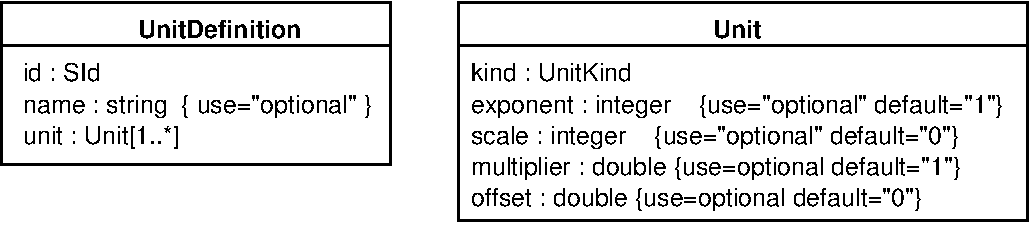
\includegraphics[scale=0.68]{graphics/unitdefinition}
  \caption{SBML Level 2's UnitDefinition and Unit.}
  \label{fig:unit-definition}
\end{figure}

To help manage this containment relationship, three standard functions are
provided by \libsbml{}: \method{XXX\_addYYY()}, \method{XXX\_getYYY()} and
\method{XXX\_getNumYYY()}.  For example, the methods for UnitDefinition
are:


\begin{methoddef}{void UnitDefinition\_addUnit (UnitDefinition\_t *ud,
Unit\_t *u)}
  Adds the given Unit to this UnitDefinition.
\end{methoddef}

\begin{methoddef}{Unit\_t *UnitDefinition\_getUnit (const UnitDefinition\_t
*ud, unsigned int n)}
Returns the nth Unit of this UnitDefinition.
\end{methoddef}

\begin{methoddef}{unsigned int UnitDefinition\_getNumUnits (const
UnitDefinition\_t *ud)}
  Return the number of Units in this UnitDefinition.
\end{methoddef}


Furthering the example, creating the \class{UnitDefinition} $mmol l^-1
s^1$ with an identifer of ``\code{mmls}'', corresponding to the following SBML,

\begin{example}
<listOfUnitDefinitions>
  <unitDefinition id="mmls">
    <listOfUnits>
      <unit kind="mole"   scale="-3"/>
      <unit kind="litre"  exponent="-1"/>
      <unit kind="second" exponent="-1"/>
    </listOfUnits>
  </unitDefinition>
</listOfUnitDefinitions>
\end{example}


could be accomplished with the following C:

\begin{example}[c]
UnitDefinition_t *ud = UnitDefinition_createWith("mmls");

UnitDefinition_addUnit(ud, Unit_createWith(UNIT_KIND_MOLE  ,  1, -3) );
UnitDefinition_addUnit(ud, Unit_createWith(UNIT_KIND_LITRE , -1,  0) );
UnitDefinition_addUnit(ud, Unit_createWith(UNIT_KIND_SECOND, -1,  0) );
\end{example}


List items are numbered starting at zero.  In the case above,
\method{UnitDefinition\_getNumUnits(\variable{ud})} returns 3 and
\method{UnitDefinition\_getUnit(\variable{ud}, 1)} returns the
\emph{second} Unit structure.  (The \class{UNIT\_KIND\_XXX} enumerations
are discussed later.)

Related to lists is a set of convenience methods for creating and adding
SBML objects to a Model object in a single operation.  The rationale is
that since a Model is the top-level container for all other SBML objects,
programmers are likely to have handles to them.  Another way to construct
the above \class{UnitDefinition\_t} object, but this time inside a
\class{Model\_t}, is:


\begin{example}[c]
Model_t            *m  = Model_createWith("MyModel");
UnitDefinition_t   *ud = Model_createUnitDefinition(m);

UnitDefinition_setName(ud, "mmls");

Model_createUnit(m, Unit_createWith(UNIT_KIND_MOLE  ,  1, -3) );
Model_createUnit(m, Unit_createWith(UNIT_KIND_LITRE , -1,  0) );
Model_createUnit(m, Unit_createWith(UNIT_KIND_SECOND, -1,  0) );
\end{example}


\method{Model\_createUnit()} creates a new Unit inside the Model
\variable{m} and returns a pointer to it (in this case the result is
discarded).  The \class{Unit\_t} is added to the last
\class{UnitDefinition\_t} created.  One caveat to be aware of with these
methods is the case where no intermediate container exists; e.g., if no
\class{UnitDefinition\_t} were created above.  In that case, the call to
\method{Model\_createUnit()} does nothing.  More specifically, no
\class{Unit\_t} is created, nothing is added to the model, and \code{NULL}
is returned.

For more detailed information on lists in \libsbml{} and the
\class{ListOf\_t} utility type provided in the library, see
Appendix~\ref{app:lists}.


%-----------------------------------------------------------------------------
\subsection{Enumerations}
\label{sec:enumerations}
%-----------------------------------------------------------------------------

SBML has two enumeration types, UnitKind and RuleType (the latter only for
SBML Level~1).  These translate directly to C \texttt{enum}s with a few
support functions for equality testing and converting to and from strings.


\begin{example}[c]
typedef enum
{
    UNIT_KIND_AMPERE
  , UNIT_KIND_BECQUEREL

   /* Omitted for space */

  , UNIT_KIND_WEBER
  , UNIT_KIND_INVALID
} UnitKind_t;
\end{example}

The following are the methods available for UnitKind:

\begin{methoddef}{int UnitKind\_equals (UnitKind\_t uk1, UnitKind\_t uk2)}
  Tests for logical equality between two UnitKinds.  This function behaves
  exactly like C's \code{==} operator, except for the following two cases:

\begin{itemize}
  \item \code{UNIT\_KIND\_LITER == UNIT\_KIND\_LITRE}
  \item \code{UNIT\_KIND\_METER == UNIT\_KIND\_METRE}
\end{itemize}

  where C would yield false (since each of the above is a distinct
  enumeration value), \method{UnitKind\_equals(...)} yields true.
  Returns true (\code{!0}) if uk1 is logically equivalent to uk2, false
  (\code{0}) otherwise.
\end{methoddef}
  
\begin{methoddef}{UnitKind\_t UnitKind\_forName (const char *name)}
  Returns the UnitKind with the given name (case-insensitive).
\end{methoddef}

\begin{methoddef}{const char *UnitKind\_toString (UnitKind\_t uk)}
  Returns the name of the given UnitKind.  The caller does not own the
  returned string and is therefore not allowed to modify it.
\end{methoddef}

The last item in the enumeration, \class{UNIT\_KIND\_INVALID}, is used
whenever, as the name implies, the \class{UnitKind} is invalid or
unknown.  The corresponding string representation is ``(Invalid
UnitKind)''.  When a Unit is created, its kind field is initialized to
\class{UNIT\_KIND\_INVALID}.  Also, \method{UnitKind\_forName()} will
return \class{UNIT\_KIND\_INVALID} if the passed-in name does not
match any known \class{UnitKind}.

The same ideas apply to RuleType, except there is no need for
\method{RuleType\_equals()}.  See \shell{RuleType.h} for more information.

\emph{Implementation Note}: The internal \variable{UNIT\_KIND\_STRINGS}
table is sorted alphabetically and \class{UnitKind\_t} matches this sort
order.  Because of this, \method{UnitKind\_forName()} is able to perform a
binary search to find a matching name, making its complexity $O(log(n))$.
That is, \method{UnitKind\_forName()} is implemented efficiently.


%-----------------------------------------------------------------------------
\subsection{Abstract Classes}
\label{sec:abstract-classes}
%-----------------------------------------------------------------------------

The SBML specification defines three classes that have no representation
apart from subclasses that specialize (inherit from) them.  In OOP
parlance, these types are termed abstract.  The abstract SBML classes are
listed in Table~\vref{tab:sbml-abstract-classes}.


\begin{table}[bth]
  \small
  \centering
  \begin{tabular}{lll}
    \toprule
    \textbf{SBML Class}           & \textbf{C Class (typedef struct)} & \textbf{SBML Level}\\
    \midrule
    \emph{SBase}                  & \class{SBase\_t}                  & all \\
    \emph{Rule}                   & \class{Rule\_t}                   & all \\
    \emph{AssignmentRule}         & \class{AssignmentRule\_t}         & Level~1\\
    \emph{SimpleSpeciesReference} & \class{SimpleSpeciesReference\_t} & Level~2\\
    \bottomrule
  \end{tabular}
  \caption{Abstract SBML classes their corresponding C class.  Although all
    classes are present in \libsbml{} at the same time, some of the classes
    only have meaning for certain levels of SBML.}
  \label{tab:sbml-abstract-classes}
\end{table}


The conventions for abstract classes in the \libsbml{} API are similar to
that of other classes with a few modifications and additions.

Since abstract classes cannot be created or destroyed directly, they have
no \method{XXX\_create()} or {XXX\_free()} methods.  Instead they have
\method{XXX\_init()} and \method{XXX\_clear()} methods which subclasses use
to initialize and free their memory, respectively.  Users of the API do not
need to worry about the create and free operations on these classes.


%Figure~\vref{fig:sbase-species} shows how Species inherits from SBase in
%SBML.  Similarly, most object structures in SBML are derived from SBase,
%and consequently all contain the fields defined by SBase (

%\begin{figure}[hbt]
%  \centering
%  \includegraphics[scale=0.68]{sbase-graphics/species}
%  \label{fig:sbase-species}
%  \caption{SBML Level~1's definition of Species and its inheritance from SBase.}
%\end{figure}


%\texttt{SBase.h} defines:


%\begin{example}[c]
%/**
% * As shown below, put SBASE_FIELDS as the *first* item of any struct
% * which "is a(n)" SBML object.
% */
%#define SBASE_FIELDS       \
%  SBMLTypeCode_t typecode; \
%  unsigned int   line;     \
%  unsigned int   column;   \
%  char           *metaid;  \
%  char           *notes;   \
%  char           *annotation
%\end{example}

%The beginning of the definition of \class{Species\_t}, covering both SBML
%Level~1 and Level~2 is

%\begin{example}[c]
%typedef struct
%{
%  SBASE_FIELDS;
%  char   *name;
%  char   *compartment;
%  double  initialAmount;
%  char   *units;
%  int     boundaryCondition;
%  int     charge;
%} Species_t;
%\end{example}

%The effect is that when the library source is compiled, the first
%three fields of \class{Species} are \variable{typecode},
%\variable{notes}, and \variable{annotation}.  In fact, every class
%that inherits from \class{SBase}, i.e. all SBML classes, have these
%same first three fields.  Accessing the notes or annotation field of a
%\class{Species\_t} \variable{*s}, or any other SBML object, is the
%same as for other fields.  For example:

%\begin{example}[c]
%if (s->notes != NULL)
%{
%  printf("Notes for Species %s:\n", (s->name == NULL) ? "(null)" : s->name);
%  printf("%s", s->notes);
%}
%\end{example}

%Setting string fields requires special care to guard against memory
%leaks.  The \method{XXX\_setYYY()} methods must be used.  But,
%\class{Species} does not define either the notes or annotation fields
%and as such there are \emph{no} \method{Species\_setNotes()} or
%\method{Species\_setAnnotation()} methods.  Instead, \class{SBase}
%defines them:


%-----------------------------------------------------------------------------
\subsection{Fields Inherited from SBase}
\label{sec:inherited-from-sbase}
%-----------------------------------------------------------------------------

Every major structure in SBML is derived from an abstract base type called
SBase.  Figure~\vref{fig:sbase} shows the pseudo-UML definition of SBase
itself, while Figure~\vref{fig:top-level} shows the overall inheritance
hierarchy of SBML.  In addition to the relationships shown in
Figure~\ref{fig:top-level}, all substructures such as \attrib{trigger} on
\class{Event} and the \class{listOf}\rule{0.5in}{0.5pt} lists in SBML are
also derived from \class{SBase}.

\begin{figure}[hbt]
  \centering
  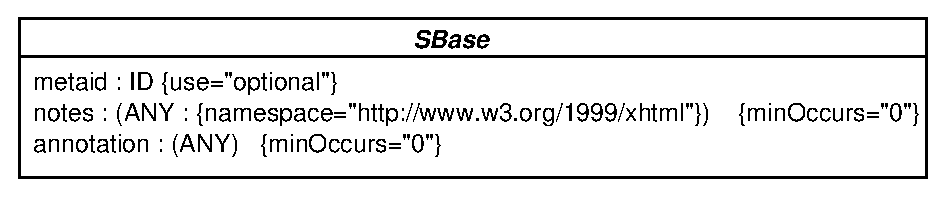
\includegraphics[scale = 0.7]{graphics/sbase}
  \caption{The definition of \class{SBase} in SBML Level~2.  See the SBML
    specifications for an explanation of the notation.}
  \label{fig:sbase}
\end{figure}


\begin{figure}[hbt]
  \centering
  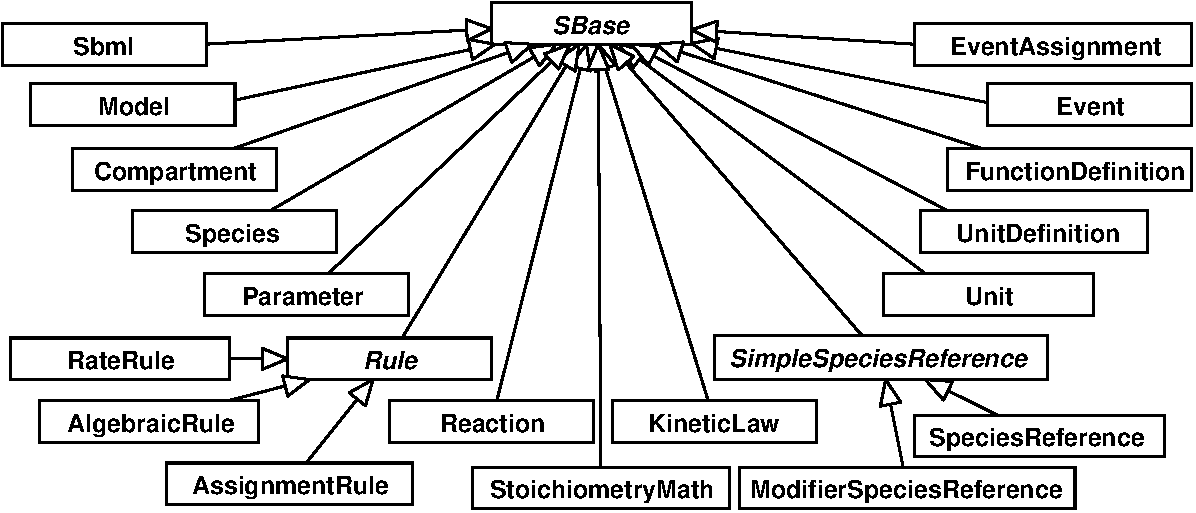
\includegraphics[scale = 0.7]{graphics/top-level}
  \caption{A UML diagram of the inheritance hierarchy of major data types
    in SBML.  Open arrows indicate inheritance, pointing from inheritors to
    their parents.  In addition to these types, all substructures in SBML
    (including, for example, all the \class{listOf} lists) are also derived
    from \class{SBase}.}
  \label{fig:top-level}
\end{figure}


The practical implication is that every class has methods for working with
the \variable{metaid}, \variable{notes} and \variable{annotation} fields.
However, the methods to work with these fields in \libsbml{} are generic:


\begin{methoddef}{const char * SBase\_getMetaId (const SBase\_t *sb)}
  Returns the \attrib{metaid} field for this SBML object.
\end{methoddef}


\begin{methoddef}{const char * SBase\_getNotes (const SBase\_t *sb)}
  Returns the \attrib{notes} field for this SBML object.
\end{methoddef}


\begin{methoddef}{const char * SBase\_getAnnotation (const SBase\_t *sb)}
  Returns the \attrib{annotation} field for this SBML object.
\end{methoddef}


\begin{methoddef}{unsigned int SBase\_getColumn (const SBase\_t *sb)}
  Returns the column number for this SBML object.
\end{methoddef}


\begin{methoddef}{unsigned int SBase\_getLine (const SBase\_t *sb)}
  Returns the line number for this SBML object.
\end{methoddef}


\begin{methoddef}{int SBase\_isSetMetaId (const SBase\_t *sb)}
  Returns \code{1} if the \attrib{metaid} for this SBML object has been
  set, \code{0} otherwise.
\end{methoddef}


\begin{methoddef}{int SBase\_isSetNotes (const SBase\_t *sb)}
  Returns \code{1} if the \attrib{notes} for this SBML object has been set,
  \code{0} otherwise.
\end{methoddef}


\begin{methoddef}{int SBase\_isSetAnnotation (const SBase\_t *sb)}
  Returns \code{1} if the \attrib{annotation} for this SBML object has been
  set, \code{0} otherwise.
\end{methoddef}


\begin{methoddef}{void SBase\_setMetaId (SBase\_t *sb, const char *metaid)}
  Sets the \attrib{metaid} field of the given SBML object to a copy of
  metaid.  If object already has a metaid, the existing string is freed
  before the new one is copied.
\end{methoddef}


\begin{methoddef}{void SBase\_setNotes (SBase\_t *sb, const char *notes)}
  Sets the notes field of the given SBML object to a copy of notes.  If
  object already has notes, the existing string is freed before the new
  one is copied.
\end{methoddef}


\begin{methoddef}{void SBase\_setAnnotation (SBase\_t *sb, const char *annotation)}
  Sets the annotation field of the given SBML object to a copy of
  annotations.  If object already has an annotation, the existing string
  is freed before the new one is copied.
\end{methoddef}


\begin{methoddef}{void SBase\_unsetMetaId (SBase\_t *sb)}
  Unsets the metaid for this SBML object.
\end{methoddef}


\begin{methoddef}{void SBase\_unsetNotes (SBase\_t *sb)}
  Unsets the notes for this SBML object.
\end{methoddef}


\begin{methoddef}{void SBase\_unsetAnnotation (SBase\_t *sb)}
  Unsets the annotation for this SBML object.
\end{methoddef}


The first argument to these functions is, of course, an object of type
SBase.  Since Species inherits from SBase, i.e., \class{Species\_t}
\emph{is an} SBase, it can be used as the first argument to these
functions.  Beware, however, that a cast is required.  For example, to set
the notes field of some \class{Species} held in variable \variable{s}, cast
the variable to type \class{SBase\_t}:

\begin{example}[c]
SBase_setNotes( (SBase_t *) s, "My Favorite Species" );
\end{example}

The same applies to all other SBML objects.

The handling of \class{annotation} elements merits further explanation.
The function \method{SBase\_getAnnotation()}, listed above, returns the
entire annotation string attached to an SBML data object, \emph{including}
the opening \texttt{<annotation>} XML element.  This is useful when reading
SBML model files because it gives access to any XML namespaces defined on
the annotation element.  For example, if a model had the following on a
structure,

\begin{example}[html]
<annotation xmlns:mstb="http://www.sbml.org/2001/ns/matlab-sbmltoolbox">
  <mstb:timestamp>2004-May-13 10:30 PST</mstb:timestamp>
  <mstb:message>These are my annotations</mstb:message>
</annotation>
\end{example}

then \method{SBase\_getAnnotation()} would return all of the above as one
string.  (In other words, it would not return simply what is being the
\texttt{<annnotation> </annotation} tags.  Similarly, when creating/setting
an annotation, programs should pass the entire annotation string including
the opening \texttt{<annotation>} element to
\method{SBase\_setAnnotation()}.  Here is an example C program setting the
same annotation string as in the example above:

\begin{example}[c]
const char *annotation =
    "<annotation xmlns:mstb=\"http://www.sbml.org/2001/ns/matlab-sbmltoolbox\">"
    "  <mstb:timestamp>2004-May-13 10:30 PST</mstb:timestamp>\n"
    "  <mstb:message>These are my annotations</mstb:message>\n"
    "</annotation>";

SBase_setAnnotation(model, annotation);
\end{example}



%-----------------------------------------------------------------------------
\subsection{Typecodes}
\label{sec:typecodes}
%-----------------------------------------------------------------------------

Each SBML class has a \variable{typecode} that is initialized when
an object is instantiated.  The \variable{typecode} is a simple C
enumeration, defined in \shell{SBMLTypeCodes.h} (which is included by the
main \libsbml{} include file, \shell{SBMLTypes.h}, so client code does not
need to include it separately):

\begin{example}[c]
/**
 * An enumeration of SBML Level 2 types to help identify SBML objects at runtime.
 * Abstract types do not have a typecode since they cannot be instantiated.
 */
typedef enum
{
    SBML_COMPARTMENT
  , SBML_DOCUMENT
  , SBML_EVENT
  , SBML_EVENT_ASSIGNMENT
  , SBML_FUNCTION_DEFINITION
  , SBML_KINETIC_LAW
  , SBML_LIST_OF
  , SBML_MODEL
  , SBML_PARAMETER
  , SBML_REACTION
  , SBML_SPECIES
  , SBML_SPECIES_REFERENCE
  , SBML_MODIFIER_SPECIES_REFERENCE
  , SBML_UNIT_DEFINITION
  , SBML_UNIT
  , SBML_ALGEBRAIC_RULE
  , SBML_ASSIGNMENT_RULE
  , SBML_RATE_RULE
  , SBML_SPECIES_CONCENTRATION_RULE
  , SBML_COMPARTMENT_VOLUME_RULE
  , SBML_PARAMETER_RULE
} SBMLTypeCode_t;
\end{example}

The primary reason for the \variable{typecode} is distinguish specific
types of rules in a Model.  A \class{Model\_t} contains a list of rules,
but a \class{Rule\_t} in SBML Level~1 may be of one of four specific types:
\class{AlgebraicRule}, \class{SpeciesConcentrationRule},
\class{CompartmentVolumeRule} and \class{ParameterRule}.  Having a type
code associated with each object allows calling programs to distinguish its
type.  Without type codes, it would be impossible.


%=============================================================================
\section{Reading and Writing SBML Files}
\label{sec:reading-sbml}
%=============================================================================

SBML may be read from a file or an in memory string into an
SBMLDocument.  \libsbml{} defines two basic read functions:

\begin{methoddef}{SBMLDocument\_t *readSBML (const char *filename)}
  Reads the SBML document from the file named by \variable{filename} and
  returns a pointer to it.
\end{methoddef}

\begin{methoddef}{SBMLDocument\_t *readSBMLFromString (const char *xml)}
  Reads the SBML document from the given XML string and returns a pointer
  to it.
  The XML string must be complete and legal XML document.  Among other
  things, it must start with an XML processing instruction.  For example,
  \begin{example}
    <?xml version='1.0' encoding='UTF-8'?>
  \end{example}
\end{methoddef}


These functions return a pointer to an \class{SBMLDocument\_t} object.
This object represents the whole SBML model; it corresponds to the
\class{Sbml} class object in the SBML Level~2 specification, but does not
have a direct correspondence in SBML Level~1.  (But, it is created by
\libsbml{} no matter whether the model is Level~1 or Level~2.)

\class{SBMLDocument\_t} in Level~2 is derived from SBase, so that it
contains the usual SBase fields of \attrib{metaid}, \attrib{notes} and
\attrib{annotation}, as well as two other fields defined by \class{Sbml}:
\attrib{level} and \attrib{version}.  The following methods provide access
to information about the level and version of the SBML input:


\begin{methoddef}{unsigned int SBMLDocument\_getLevel (const SBMLDocument\_t *d)}
  Returns the SBML level of this SBML document.
\end{methoddef}


\begin{methoddef}{unsigned int SBMLDocument\_getVersion (const SBMLDocument\_t *d)}
  Returns the SBML version of this SBML document.
\end{methoddef}


Of course, the whole point of reading an SBML file or data stream is to get
at the SBML model it contains.  The following method allows access to the
Model object within an SBML document:


\begin{methoddef}{Model\_t * SBMLDocument\_getModel (const SBMLDocument\_t *d)}
  Returns the Model associated with this \class{SBMLDocument\_t} object.
\end{methoddef}


\libsbml{} stores warnings and error messages that may be encountered while
parsing the XML input.  Each warning or error is a \class{ParseMessage\_t}
object.  To access the lists of diagnostic messages in an
\class{SBMLDocument\_t} object, use the following methods:


\begin{methoddef}{ParseMessage\_t *SBMLDocument\_getWarning
(SBMLDocument\_t *d, unsigned int n)}
   Returns the nth warning encountered during the parse of this
   SBMLDocument or \code{NULL} if \code{n > getNumWarnings() - 1}.
 \end{methoddef}

\begin{methoddef}{ParseMessage\_t *SBMLDocument\_getError (SBMLDocument\_t *d,
unsigned int n);}
   Returns the nth error encountered during the parse of this
   SBMLDocument or \code{NULL} if \code{n > getNumErrors() - 1}.
 \end{methoddef}

\begin{methoddef}{ParseMessage\_t *SBMLDocument\_getFatal (SBMLDocument\_t *d,
unsigned int n)}
   Returns the nth fatal error encountered during the parse of this
   SBMLDocument or \code{NULL} if \code{n > getNumErrors() - 1}.
 \end{methoddef}


\begin{methoddef}{unsigned int SBMLDocument\_getNumWarnings
(SBMLDocument\_t *d)}
   Returns the number of warnings encountered during the parse of this
   SBMLDocument.
 \end{methoddef}

\begin{methoddef}{unsigned int SBMLDocument\_getNumErrors (SBMLDocument\_t *d)}
   Returns the number of errors encountered during the parse of this
   SBMLDocument.
 \end{methoddef}

\begin{methoddef}{unsigned int SBMLDocument\_getNumFatals (SBMLDocument\_t *d)}
   Returns the number of fatal errors encountered during the parse of this
   SBMLDocument.
 \end{methoddef}
  

\begin{methoddef}{void SBMLDocument\_printWarnings (SBMLDocument\_t *d,
FILE *stream)}
  Prints all warnings encountered during the parse of this SBMLDocument to
  the given \variable{stream}.  If no warnings have occurred, i.e.
  \code{SBMLDocument\_getNumWarnings(d) == 0}, no output will be sent to
  \variable{stream}. The format of the output is:
  \begin{example}
    %d Warning(s):
      Line %d, Col %d: %s
      ...
  \end{example}
  This is a convenience function to aid in debugging.  For example:\\
  \code{SBMLDocument\_printWarnings(d, stdout)}.
 \end{methoddef}
  

\begin{methoddef}{void SBMLDocument\_printErrors (SBMLDocument\_t *d,
FILE *stream)}
  Prints all errors encountered during the parse of this SBMLDocument
  to the given \variable{stream}.  If no errors have occurred, that is, if 
  \code{SBMLDocument\_getNumErrors(d) == 0}, no output will be sent
  to \variable{stream}. The format of the output is:
  \begin{example}
    %d Error(s):
      Line %d, Col %d: %s
      ...
  \end{example}
  This is a convenience function to aid in debugging.  For example:\\
  \code{SBMLDocument\_printErrors(d, stdout)}.
 \end{methoddef}
  

\begin{methoddef}{void SBMLDocument\_printFatals (SBMLDocument\_t *d,
FILE *stream)}
  Prints all fatals encountered during the parse of this SBMLDocument
  to the given \variable{stream}.  If no fatals have occurred, that is, if
  \code{SBMLDocument\_getNumFatals(d) == 0}, no output will be sent
  to \variable{stream}. The format of the output is:
  \begin{example}
    %d Fatal(s):
      Line %d, Col %d: %s
      ...
  \end{example}
  This is a convenience function to aid in debugging.  For example:\\
  \code{SBMLDocument\_printFatals(d, stdout)}.
 \end{methoddef}

There are a few other methods defined by \method{SBMLDocument\_t}, but
their discussion is left to Section~\ref{sec:sbml-levels}


%-----------------------------------------------------------------------------
\subsection{A Simple Example of Reading SBML}
\label{sec:read-example}
%-----------------------------------------------------------------------------

The following example is included in the \libsbml{} distribution as
\shell{readSBML.c} in the subdirectory \shell{examples}.  It is not
compiled as part of the normal build process, but a Makefile is provided in
the \shell{examples} subdirectory that can be used to build
\shell{readSBML.c} and other examples.  Once \libsbml{} itself is
installed, you should be able to compile the examples by simply typing the
following command in the \shell{examples} directory:

\begin{example}[csh]
  make
\end{example}

The \shell{readSBML} program takes a single command-line argument, the name
of an SBML file, reads it into memory and reports some basic information
about the file and any warnings or errors generated by \libsbml{} while
parsing the file.  Here is an example of using it on some of the sample
SBML files provided in the \shell{src/test-data} subdirectory of the
\libsbml{} distribution.  In this example, the current directory is assumed
to be \shell{examples}.

\begin{example}[csh]
  ./readSBML ../src/test-data/l1v1-branch.xml
  ./readSBML ../src/test-data/l1v1-minimal.xml
  ./readSBML ../src/test-data/l1v1-rules.xml
  # etc...
\end{example}


The complete text of \shell{readSBML} is shown in Figure~\vref{fig:printsbml}.

\begin{figure}
\begin{codeVerbatim}[C,flexiblecolumns=false]
#include <stdio.h>

#include "sbml/SBMLTypes.h"

int
main (int argc, char *argv[])
{
  SBMLDocument_t *d;
  Model_t        *m;

  unsigned int level, version;


  if (argc != 2)
  {
    printf("\n  usage: printSBML <filename>\n\n");
    return 1;
  }

  d = readSBML(argv[1]);
  m = SBMLDocument_getModel(d);

  level   = SBMLDocument_getLevel  (d);
  version = SBMLDocument_getVersion(d);

  printf("\n");
  printf("File: %s (Level %u, version %u)\n", argv[1], level, version);

  printf("         ");
  if (level == 1)
  {
    printf("model name: %s\n", Model_getName(m));
  }
  else
  {
    printf("  model id: %s\n", 
           Model_isSetId(m) ? Model_getId(m) : "(empty)");
  }

  printf("functionDefinitions: %d\n", Model_getNumFunctionDefinitions(m));
  printf("    unitDefinitions: %d\n", Model_getNumUnitDefinitions(m)    );
  printf("       compartments: %d\n", Model_getNumCompartments(m)       );
  printf("            species: %d\n", Model_getNumSpecies(m)            );
  printf("         parameters: %d\n", Model_getNumParameters(m)         );
  printf("          reactions: %d\n", Model_getNumReactions(m)          );
  printf("              rules: %d\n", Model_getNumRules(m)              );
  printf("             events: %d\n", Model_getNumEvents(m)             );
  printf("\n");

  SBMLDocument_printWarnings(d, stdout);
  SBMLDocument_printErrors  (d, stdout);
  SBMLDocument_printFatals  (d, stdout);

  SBMLDocument_free(d);
  return 0;
}
\end{codeVerbatim}
\caption{The text of the program \shell{printSBML.c} provided in the
  \shell{examples} subdirectory of the \libsbml{} distribution.}
\label{fig:printsbml}
\end{figure}
                                        

%-----------------------------------------------------------------------------
\subsection{XML Schema Validation}
\label{sec:schema-validation}
%-----------------------------------------------------------------------------

To have \libsbml{} validate an SBML document against an SBML (XML) Schema
when using a Schema-aware parser such as Xerces requires creating an
\texttt{SBMLReader} object and setting the appropriate schema filename and
validation level.  The functions for doing this are:


\begin{methoddef}{SBMLReader\_t *SBMLReader\_create (void)}
  Creates a new SBMLReader and returns a pointer to it.  By default
  schema validation is off (\texttt{XML\_SCHEMA\_VALIDATION\_NONE})
  and \texttt{schemaFilename} is \texttt{NULL}.
\end{methoddef}


\begin{methoddef}{void SBMLReader\_free (SBMLReader\_t *sr)}
  Frees the given SBMLReader.
\end{methoddef}


\begin{methoddef}{void SBMLReader\_setSchemaFilenameL1v1 (SBMLReader\_t *sr, const char *filename)}
  Sets the file containing the XML Schema used by this SBMLReader to
  validate SBML Level~1 Version~1 documents.  The \variable{filename}
  should be either (1) an absolute path or (2) a path relative to the
  directory containing the SBML file(s) to be read.
\end{methoddef}


\begin{methoddef}{void SBMLReader\_setSchemaFilenameL1v2 (SBMLReader\_t *sr, const char *filename)}
  Sets the file containing the XML Schema used by this SBMLReader to
  validate SBML Level~1 Version~2 documents.  The \variable{filename}
  should be either (1) an absolute path or (2) a path relative to the
  directory containing the SBML file(s) to be read.
\end{methoddef}


\begin{methoddef}{void SBMLReader\_setSchemaFilenameL2v1 (SBMLReader\_t *sr, const char *filename)}
  Sets the file containing the XML Schema used by this SBMLReader to
  validate SBML Level~2 Version~1 documents.  The \variable{filename}
  should be either (1) an absolute path or (2) a path relative to the
  directory containing the SBML file(s) to be read.
\end{methoddef}


\begin{methoddef}{void SBMLReader\_setSchemaValidationLevel (SBMLReader\_t *sr,
XMLSchemaValidation\_t level)}
  Sets the level of schema validation used by this SBMLReader.
  The possible values for \variable{level} are:
  \begin{itemize}
  \item \code{XML\_SCHEMA\_VALIDATION\_NONE} (\code{0}) turns schema
    validation off.
    
  \item \code{XML\_SCHEMA\_VALIDATION\_BASIC} (\code{1}) validates an XML
    instance document against an XML Schema.  Those who wish to perform
    schema checking on SBML documents should use this option.
    
  \item \code{XML\_SCHEMA\_VALIDATION\_FULL} (\code{2}) validates both the
    instance document itself \emph{and} the XML Schema document.  The XML
    Schema document is checked for violation of particle unique attribution
    constraints and particle derivation restrictions, which is both
    time-consuming and memory intensive.  Few users will be interested in
    this. 
  \end{itemize}
\end{methoddef}

Note that the \method{SBMLReader\_setXYZ} methods above have no effect when
using a parser such as Expat, because it is not a validating XML parser and
the settings have no meaning for it.

Once an \class{SBMLReader\_t} object has been created, two variants of the
functions \method{readSBML()} and \method{readSBMLFromString()} previously
discussed in Section~\ref{sec:reading-sbml} become available.  These
variants can be thought of as methods of the \class{SBMLReader\_t} class:


\begin{methoddef}{SBMLDocument\_t *SBMLReader\_readSBML (SBMLReader\_t *sr,
const char *filename)}
Reads the SBML document using the \class{SBMLReader\_t} object passed in
argument \variable{sr} from the given \variable{filename} and returns a
pointer to it.
\end{methoddef}

\begin{methoddef}{SBMLDocument\_t *SBMLReader\_readSBMLFromString (SBMLReader\_t *sr,\\
const char *xml)}
Reads the SBML document using the \class{SBMLReader\_t} object passed in
argument \variable{sr} from the character string passed in variable
\variable{xml} and returns a pointer to it.  The XML string in
\variable{xml} must be complete and legal XML document.  Among other
things, it must start with an XML processing instruction, i.e.,
  \begin{example}
    <?xml version='1.0' encoding='UTF-8'?>
  \end{example}
\end{methoddef}


Schema violations are reported in the \class{SBMLDocument\_t}'s list of
\class{ParseMessages\_t}, according to the principles discussed in
Section~\ref{sec:reading-sbml}.


%-----------------------------------------------------------------------------
\subsection{Writing SBML Files}
\label{sec:writing-sbml}
%-----------------------------------------------------------------------------

Writing SBML is, in the end, a very simple matter in \libsbml{}.  The
library provides the following two methods for this purposes.


\begin{methoddef}{int writeSBML (SBMLDocument\_t *d, \\const char *filename)}
  Writes the given SBML document to the given \variable{filename}.  Returns
  \code{1} on success and \code{0} on failure (e.g., if the file named by
  \variable{filename} could not be opened for writing).
\end{methoddef}


\begin{methoddef}{char *writeSBMLToString (SBMLDocument\_t *d)}
  Writes the given SBML document to an in-memory string and returns a
  pointer to it.  The string is owned by the caller and should be freed
  (with \code{free()}) when no longer needed.  Returns \code{NULL} on
  failure.
\end{methoddef}



%=============================================================================
\section{Handling of Mathematical Formulas and MathML}
\label{sec:mathml}
%=============================================================================

\libsbml{} can read and write MathML 2.0~\citep{ausbrooks_2001b} content in
SBML documents and data streams, as well as translate between MathML and
the text-string formulas used in SBML Level~1.  This section describes the
library's capabilities for handling MathML and mathematics.

%-----------------------------------------------------------------------------
\subsection{Reading and Writing Formulas in Text-String Form}
\label{sec:text-string-math}
%-----------------------------------------------------------------------------

In SBML Level~1, mathematical formulas are expressed as text strings using
a simple C-like syntax.  In SBML Level~2, mathematical formulas are
expressed in MathML syntax.  \libsbml{} helps calling programs smooth over
this difference by providing an API that allows working with formulas in
both text-string and MathML form, and to interconvert mathematical
expressions between these forms (to the extent possible by the differences
between SBML Levels~1 and~2.)

Formulas in \libsbml{} are represented internally using Abstract Syntax
Trees (ASTs).  ASTs are described in detail in Appendix~\ref{app:ast}.
When \libsbml{} reads an SBML model, it converts the expressions into ASTs
and stores the ASTs in the corresponding data structures that have
mathematical formulas (such as in an SBML KineticLaw).  Thus, the
\method{KineticLaw\_getMath()} method, for example, returns a pointer to
the root of an AST corresponding to the formula stored there.

Many software packages provide users with the ability to express formulas
for such things as reaction rate expressions, and these packages'
interfaces often let users type in the formulas directly as strings.
\libsbml{} provides two high-level functions for working with mathematical
expressions in the form of strings: \method{SBML\_parseFormula()} and
\method{SBML\_formulaToString()}.

\begin{methoddef}{ASTNode\_t *SBML\_parseFormula (const char *formula)}
  Parses the given string as a mathematical formula in SBML Level~1 syntax
  form, and returns a representation of it as an Abstract Syntax Tree
  (AST).  This function returns the root node of the AST.  If the formula
  contains a syntax error, this function returns \code{NULL} instead.
\end{methoddef}

\begin{methoddef}{char *SBML\_formulaToString (ASTNode\_t *tree)}
  Returns a text-string mathematical expression corresponding to the
  Abstract Syntax Tree given as the argument.  The caller owns the memory
  allocated for the returned string and is responsible for freeing it when
  it is no longer needed.
\end{methoddef}

Using these methods is easy.  The following is a code fragment that
illustrates calling the parser function repeatedly with different formula
strings, taking the ASTs returned each time and handing them back to the
formula generator and comparing the strings to make sure they matched.
(This is not something a real application would ever need to do, but it
does simply illustrate the use of these two methods.)

\begin{example}[c]
const char *formulae[] =
{
  "1",
  "2.1",
  "2.1e+10",
  "foo",
  "1 + foo",
  "1 + 2",
  "1 + 2 * 3",
  "(1 - 2) * 3",
  "1 + -2 / 3",
  "1 + -2e-100 / 3",
  "1 - -foo / 3",
  "2 * foo^bar + 3.1",
  "foo()",
  "foo(1)",
  "foo(1, bar)",
  "foo(1, bar, 2^-3)",
  ""
};

ASTNode_t *n;
char      *s;
int        i;

for (i = 0; i < *formulae[i]; i++)
{
  n = SBML_parseFormula( formulae[i] );  /* Convert string to AST */
  s = SBML_formulaToString(n);           /* Convert AST back to string */

  if ( strcmp(s, formulae[i]) != 0 ) 
  {
    printf("Formula '%s' parsed incorrectly\n", formulae[i] );
  }

  ASTNode_free(n);
  free(s);
}
\end{example}

Section~\ref{sec:mathml-special-cases} describes some additional points
that are worth knowing about the mathematical formula handling in
\libsbml{}.  For example,  Level~1 formula strings and Level~2 MathML
expressions can  be interconverted.


%-----------------------------------------------------------------------------
\subsection{Reading Formulas in MathML Form: \class{MathMLDocument\_t} and ASTs}
\label{sec:mathml-math}
%-----------------------------------------------------------------------------

There may arise situations in which an application needs to convert MathML
directly into an AST.  \libsbml{} provides the utility function
\method{readMathMLFromString()} for this purpose:

\begin{methoddef}{MathMLDocument\_t *readMathMLFromString (const char *xml)}
  Reads a string containing an XML MathML expression, constructs the
  corresponding Abstract Syntax Tree and returns a pointer to a
  \class{MathMLDocument\_t} object holding the tree structure.
\end{methoddef}

The object returned by \method{readMathMLFromString()} is a simple
container for an AST.  The class of this object, MathMLDocument, is not
defined by the SBML language standard but is provided in \libsbml{} as a
utility class.  MathMLDocument serves as a top-level container for XML
documents containing only MathML; in some ways it mirrors the SBMLDocument
class, which acts as a container for XML documents containing SBML.  The
definition of \class{MathMLDocument\_t} is as follows:
 
\begin{example}[c]
/**
 * The MathMLDocument
 */
typedef struct
{
  ASTNode_t *math;
} MathMLDocument_t;
\end{example}  

The following are the functions defined for the MathMLDocument class:

\begin{methoddef}{MathMLDocument\_t *MathMLDocument\_create ()}
  Creates a \class{MathMLDocument\_t} object.
\end{methoddef}

\begin{methoddef}{void MathMLDocument\_free (MathMLDocument\_t *d)}
  Frees the given \class{MathMLDocument\_t} object.
\end{methoddef}

\begin{methoddef}{ASTNode\_t *MathMLDocument\_getMath (const MathMLDocument\_t *d)}
  Returns the Abstract Syntax Tree representation of the mathematical
  formula stored in this \class{MathMLDocument\_t} object.
\end{methoddef}

\begin{methoddef}{int MathMLDocument\_isSetMath (const MathMLDocument\_t *d)}
  Returns \code{1} if the math of this MathMLDocument has been set, \code{0}
  otherwise.
\end{methoddef}

\begin{methoddef}{void MathMLDocument\_setMath (MathMLDocument\_t *d, ASTNode\_t *math)}
  Sets the math of this MathMLDocument to the given AST node.  The node
  \textbf{is not copied} and this MathMLDocument \textbf{takes ownership}
  of it; i.e., subsequent calls to this function or a call to
  \method{MathMLDocument\_free()} will free the AST node (and any child
  nodes attached to it).
\end{methoddef}

Note that because the content passed to \method{readMathMLFromString()} is
handed to an XML parser, the string given as argument must be a complete
XML (though not necessarily SBML) document.  The following example
illustrates the use of this function with a valid MathML input.

\begin{example}[c]
MathMLDocument_t *doc;
ASTNode_t          *ast;
char               *result;

const char* s = "<?xml version='1.0' encoding='UTF-8'?>"
                  "<math xmlns='http://www.w3.org/1998/Math/MathML'>"
                    "<apply><arccos/><ci> x </ci></apply>"
                  "</math>";

doc    = readMathMLFromString(s);
ast    = MathMLDocument_getMath(doc);
\end{example}

The code above would create an AST structure stored in the variable
\code{ast}.  This tree structure could then be inspected using the AST node
methods described in Appendix~\ref{app:ast}.

Finally, \libsbml{} provides two utility methods for writing out MathML
represented in ASTs.  Both of the following take a
\class{MathMLDocument\_t} class object, convert the expression tree stored
there, and write out the appropriate text in MathML syntax.


\begin{methoddef}{int writeMathML (MathMLDocument\_t *d, const char *filename)}
  Writes the given MathML document to filename.  Returns \code{1} on
  success and \code{0} on failure (e.g., if \variable{filename} could not
  be opened for writing or the MathMLWriter character encoding is invalid).
\end{methoddef}


\begin{methoddef}{char * writeMathMLToString (MathMLDocument\_t *d)}
  Writes the given MathML document to an in-memory string and returns a
  pointer to it.  The string returned is owned by the caller and should be
  freed (with \code{free()}) when no longer needed.  Returns \code{NULL} on
  failure
\end{methoddef}



%-----------------------------------------------------------------------------
\subsection{Differences between SBML Level~1 Formulas and MathML}
\label{sec:function-names}
%-----------------------------------------------------------------------------

The text-string based mathematical formula syntax of SBML Level~1 is
\emph{mostly} compatible with the representation of formulas in MathML.  A
few differences exist in the names of predefined functions such as
\code{arccos}.  Table~\vref{tab:function-names} gives the mapping
between SBML Level~1 and Level~2 function names.  

\begin{table}[bth]
  \small
  \centering
  \ttfamily
  \begin{tabular}{ll}
    \toprule
    \textrm{\textbf{SBML Level 1}} & \textrm{\textbf{SBML Level 2}} \\
    \midrule
    abs     & abs \\
    acos    & \underline{arccos} \\
    asin    & \underline{arcsin} \\
    atan    & \underline{arctan} \\
    ceil    & \underline{ceiling} \\
    cos     & cos \\
    exp     & exp \\
    floor   & floor \\
    log     & \underline{ln} \\
    log10(x) & \underline{log(10, x)} \\
    pow(x, y) &       \underline{power(x, y)} \\
    sqr(x)  & \underline{power(x, 2)} \\
    sqrt(x) & \underline{root(2, x)} \\
    sin     & sin \\
    tan     & tan \\
    \bottomrule
  \end{tabular}
  \caption{Basic mathematical functions defined in SBML Levels~1 and~2.
The underlined functions are different between the two levels of SBML.}
  \label{tab:function-names}
\end{table}

%-----------------------------------------------------------------------------
\subsection{Additional Notes about the Handling of Mathematical Formulas}
\label{sec:mathml-special-cases}
%-----------------------------------------------------------------------------

The \libsbml{} formula parser has been carefully engineered so that
transformations from MathML to infix string notation \emph{and back} is
possible with a minimum of disruption to the structure of the mathematical
expression.

Figure~\vref{fig:eg-round-trip} shows a simple program that, when run,
takes a MathML string compiled into the program, converts it to an AST,
converts \emph{that} to an infix representation of the formula, compares it
to the expected form of that formula, and finally translates that formula
back to MathML and displays it.  The output displayed on the terminal
should have the same structure as the MathML it started with.  The program
is a simple example of using the various MathML and AST reading and writing
methods, and shows that \libsbml{} preserves the ordering and structure of
the mathematical expressions.


\begin{figure}[b]
  \begin{codeVerbatim}[C,flexiblecolumns=false]
#include <stdio.h>
#include <string.h>
#include "sbml/SBMLTypes.h"

int
main (int argc, char *argv[])
{
    MathMLDocument_t *doc;
    ASTNode_t        *ast;
    char             *result;
    MathMLDocument_t *new_doc;
    ASTNode_t        *new_mathml;
    char             *new_s;

    const char* expected = "1 + f(x)";

    const char* s = "<?xml version='1.0' encoding='UTF-8'?>"
        "<math xmlns='http://www.w3.org/1998/Math/MathML'>"
        "  <apply> <plus/> <cn> 1 </cn>"
        "                  <apply> <ci> f </ci> <ci> x </ci> </apply>"
        "  </apply>"
        "</math>";

    doc    = readMathMLFromString(s);
    ast    = MathMLDocument_getMath(doc);
    result = SBML_formulaToString(ast);

    if ( strcmp(result, expected) == 0 ) 
    {
        printf("Got expected result\n");
    }
    else
    {
        printf("Mismatch after readMathMLFromString()\n");
    }

    new_mathml = SBML_parseFormula(result);
    new_doc    = MathMLDocument_create();
    MathMLDocument_setMath(new_doc, new_mathml);
    new_s      = writeMathMLToString(new_doc);

    printf("Result of writing AST:\n");
    printf(new_s);

    return 0;
}
  \end{codeVerbatim}
  \caption{Short program to translate MathML into a formula string and back.}
  \label{fig:eg-round-trip}
\end{figure}

The string form produced by \method{SBML\_formulaToString()} and written by
\method{writeMathMLToString()} is in SBML Level~1 formula string syntax, a
simple C-inspired infix notation defined in the SBML Level~1
specification~\cite{hucka_2001b}.  It can therefore be handed to a program
that understands SBML Level~1 mathematical expressions, or used as part of
a translation system.  The \libsbml{} distribution comes with an example
program in the \shell{examples} subdirectory called \shell{translateMath}
that implements an interactive command-line demonstration of translating
infix formulas into MathML and vice-versa.

\libsbml{} offers the ability to translate entire SBML Level~1 models to
SBML Level~2, as explained below, and hopefully in the future will also
provide the ability to translate a subset of Level~2 models to Level~1
(though this latter capability is not yet implemented).


%=============================================================================
\section{Levels of SBML}
\label{sec:sbml-levels}
%=============================================================================

At the time of this writing, there exist 3 flavors of SBML: Level~1
Versions~1 and~2, and SBML Level~2 Version~1.  A software application may
need to read and/or write any of these versions, depending on its purpose.
\libsbml{} provides support for all three definitions of SBML.

Along with the methods discussed in Section~\ref{sec:reading-sbml}, the
\class{SBMLDocument\_t} object class also defines the following methods
that impact how a model is written out:


\begin{methoddef}{void SBMLDocument\_setModel (SBMLDocument\_t *d, Model\_t *m)}
  Sets the Model of this SBML document to the given \class{Model\_t} object.
  Any previously defined model in \variable{d} is unset and freed.
\end{methoddef}


\begin{methoddef}{void SBMLDocument\_setLevel (SBMLDocument\_t *d, unsigned int level)}
  Sets the level of this SBML document to \variable{level}.  Valid levels
  are currently 1 and 2. 
\end{methoddef}


\begin{methoddef}{void SBMLDocument\_setVersion (SBMLDocument\_t *d, unsigned int version)}
  Sets the version of this SBML document to the given \variable{version}
  number.  Valid versions are currently 1 and 2 for SBML Level~1 and 1 for SBML
  Level~2.
\end{methoddef}


Setting the level using \method{SBMLDocument\_setLevel()} affects the
possible fields and values available when setting and reading fields.
Certain translations take place immediately upon changing levels.  For
example, if one starts with a Level~1 model and then calls
\method{SBMLDocument\_setLevel()} to set the level to 2, the model
structure at that moment is translated internally so that such things as
object names are converted to \attrib{id}'s (which do not exist in
Level~1).

\begin{figure}[bth]
  \begin{codeVerbatim}[C,flexiblecolumns=false]
#include <stdio.h>
#include "sbml/SBMLTypes.h"

int
main (int argc, char *argv[])
{
  unsigned int errors = 0;
  SBMLDocument_t *d;

  if (argc != 3)
  {
    printf("\nusage: convertSBML <input-filename> <output-filename>\n\n");
    return 1;
  }

  d = readSBML(argv[1]);

  errors = SBMLDocument_getNumWarnings(d) + SBMLDocument_getNumErrors(d) +
           SBMLDocument_getNumFatals(d);

  if (errors > 0)
  {
    printf("Error(s):\n");

    SBMLDocument_printWarnings(d, stdout);
    SBMLDocument_printErrors  (d, stdout);
    SBMLDocument_printFatals  (d, stdout);

    printf("Conversion skipped.  Please correct the above and re-run.\n");
  }
  else
  {
    SBMLDocument_setLevel(d, 2);
    writeSBML(d, argv[2]);
  }

  SBMLDocument_free(d);
  return errors;
}
  \end{codeVerbatim}
  \caption{The text of the example C program \shell{convertSBML.c}.}
  \label{fig:convert-sbml}
\end{figure}


The C program listed in Figure~\ref{fig:convert-sbml} is provided in the
\libsbml{} distribution in the \shell{examples} subdirectory.  This
command-line program takes two arguments: the name of an input file and the
name of an output file.  It then translates the SBML in the input file into
SBML Level~2 and writes it out to the named output file.  It may be
surprising to see how short this program is.


%=============================================================================
\section{Validation of SBML Models}
\label{sec:sbml-validation}
%=============================================================================

\libsbml{} performs a certain amount of validation of SBML inputs at the
time of parsing files and data streams.  However, the checks performed are
mostly syntactic in nature, based on the XML Schema for SBML (and as noted
elsewhere, getting the most of this validation capability requires the
using of an XML Schema-aware parser such as Xerces).

\libsbml{} implements more extensive semantic validation rules internally.
At the time of this writing, over 30 tests are implemented.  Examples of
these rules include: compartments' \attrib{spatialSizeUnits} fields must be
consistent with their \attrib{spatialDimensions}; species with
\attrib{hasOnlySubstanceUnits} set to true must not have an
\attrib{initialConcentration}; and others.
    
Semantic validation rules in \libsbml{} (and indeed, in SBML in general)
are still somewhat experimental; for this reason, the library does not
perform them automatically.  Callers must request semantic validation to be
invoked explicitly by calling the following method.


\begin{methoddef}{unsigned int SBMLDocument\_validate (const SBMLDocument\_t *d)}
  Performs semantic validation on the document.  Calling programs can query
  the results by calling \method{SBMLDocument\_getNumWarnings()},
  \method{SBMLDocument\_getNumErrors()},
  \method{SBMLDocument\_getNumFatals()}, and related methods.  This method
  returns (as an integer) the number of semantic validation errors
  encountered
\end{methoddef}

% FIXME give more details about the number returned.  Here's what B.B. says:
%
%The validator keeps track of every rule fired (or run) and increments a
%counter if it fails.  It also logs an error message.  That error message
%(ParseMessage) is logged to the same list of error messages that XML Schema
%validation errors are logged to, i.e. the one kept by SBMLDocument.
%getNumErrors() simply returns the size of this list.  The count of violated
%rules is returned by the validator and SBMLDocument_validate() propagates
%this number to its caller.



%=============================================================================
\section{Special Considerations and Known Issues}
\label{sec:special-considerations}
%=============================================================================

This section summarizes special considerations, known issues and caveats
surrounding the use and behavior of \libsbml{}.


\subsection{Conformance to SBML}

Currently, \libsbml{} supports all of SBML Level~1 Version~1 and Version~2,
and nearly all of SBML Level~2 Version~1.  The still-unsupported parts of
the Level~2 specification are:

\begin{itemize}\setlength{\parskip}{-0.25ex}
\item Support for RDF
\item Support for MathML's \code{semantics} elements
\item Support for MathML's \code{annotation} elements
\item Support for MathML's \code{annotation-xml} elements
\end{itemize}


\subsection{Issues Related to XML Parsers}
\label{sec:issues-about-parsers}

Using Expat prevents \libsbml{} from performing XML Schema-based validation
of SBML input.  This removes a number of verification checks from the
parsing stage and may cause unexpected behavior in the face of malformed or
invalid SBML content.  Here are some implications of not performing XML
Schema validation:

\begin{itemize}

\item The syntax of identifiers (i.e., conformance to SId syntax) will not
  be verified.  This means that identifiers that are not in conformance to
  SBML SId specifications will be passed through without being flagged as
  invalid.

\item Data types of values assigned to fields in a model will not be
  verified for conformance to the SBML specification.  In some cases this
  means that those values will not be assigned to the corresponding object
  structures created by \libsbml{}.  For example, reading a model
  containing a compartment definition having a volume of \code{"mumble"} (a
  string instead of a number) will result in \libsbml{} simply ignoring the
  value and treating the input as if no value was supplied.

\item Elements present in an SBML input file or data stream, but that are
  not actually defined by the SBML specification, will not be noticed.
  (Such SBML input should be flagged as invalid, but will not be.)
  
\item XML entity references (e.g. XML's \verb|&#160;|), which are most
  likely to occur in XHTML \verb|<notes>| sections, will be output as their
  UTF-8 byte sequence instead of the more human readable entity reference.
  This is a bug in the Expat support in \libsbml{}, stemming from a
  limitation in the API of Expat.  (While Expat reads and writes UTF-8 by
  default, it comes with no APIs to manipulate or translate Unicode
  encodings.  Writing such a conversion routine and ensuring it is
  cross-platform is non-trivial.)
  
\item The methods discussed in Section~\ref{sec:schema-validation}, namely
  the \method{SBMLReader\_setSchemaFilename****()} methods and
  \method{SBMLReader\_setSchemaValidationLevel()}, have no effect.

\end{itemize}


Although it is poorly documented, SBML XML documents \textbf{must use only}
the \code{UTF-8} encoding.  Parsing a non-UTF-8 document may fail
unpredictably and this particular error may be difficult to diagnose,
because it will happen in the underlying XML parser and not \libsbml{}
itself.


%\subsection{Issues Related to Handling of Mathematics}
%\label{sec:issues-about-math}


%=============================================================================
\section{Acknowledgments}
\label{sec:acknowledgments}
%=============================================================================

Thanks to Mike Hucka for updating and editing this manual for version 2.0
of \libsbml{}.



\clearpage
\appendix
%=============================================================================
\section{Lists and \class{ListOf\_t}}
\label{app:lists}
%=============================================================================

While list-based convenience methods (e.g., \texttt{XXX\_getNumYYY()}) are
provided for every class, it is possible to access and manipulate each list
directly.  All lists are themselves objects of type \texttt{ListOf\_t}.
The full set of list methods are:


\begin{methoddef}{unsigned int ListOf\_getNumItems (const ListOf\_t *lo)}
  Returns the number of items in this list.
\end{methoddef}


\begin{methoddef}{void ListOf\_append (ListOf\_t *lo, void *item)}
  Adds item to the end of this list.
\end{methoddef}


\begin{methoddef}{void * ListOf\_get (const ListOf\_t *lo, unsigned int n)}
  Returns the nth item in this list.  If \code{n > ListOf\_getNumItems(list)},
  it returns \code{NULL}.
\end{methoddef}


\begin{methoddef}{void ListOf\_prepend (ListOf\_t *lo, void *item)}
  Adds item to the beginning of this \class{ListOf\_t} object.
\end{methoddef}


\begin{methoddef}{void * ListOf\_remove (ListOf\_t *lo, unsigned int n)}
  Removes the nth item from this list and returns a pointer to it.  If 
  \code{n > ListOf\_getNumItems(list)}, it returns \code{NULL}.
\end{methoddef}


Since UnitDefinitions maintains a list of Units, the UnitDefinition
example presented in Section~\ref{sec:lists} could also be written as:


\begin{example}[c]
UnitDefinition_t *ud = UnitDefinition_createWith("mmls");

UnitDefinition_addUnit(ud, Unit_createWith(UNIT_KIND_MOLE  ,  1, -3) );
UnitDefinition_addUnit(ud, Unit_createWith(UNIT_KIND_LITRE , -1,  0) );
UnitDefinition_addUnit(ud, Unit_createWith(UNIT_KIND_SECOND, -1,  0) );
\end{example}


However, this approach is not the preferred one.  The best reason to use
specific \method{XXX\_getYYY()} methods over the list API in \libsbml{} is
that the former are typed to specific items, whereas \method{ListOf\_get()}
returns a void pointer that must be cast to a specific type.  Moreover, the
code resulting from using the \method{XXX\_getYYY()} methods is arguably
more readable.

Although many specialized methods are available for accessing various data
objects in SBML, the list API is necessary for accessing such things as the
content of \attrib{notes} and \attrib{annotation} elements on SBML's
\attrib{listOf***} elements.  In addition, the only way to remove an item
from a list is to use the API directly.


%=============================================================================
\section{Abstract Syntax Trees and \texttt{ASTNode\_t}}
\label{app:ast}
%=============================================================================

Abstract Syntax Trees (ASTs) in \libsbml{} are a simple data structure for
storing mathematical expressions.  For many applications, the details of
ASTs are irrelevant because the applications can use the text-string based
translation functions described in Sections~\ref{sec:text-string-math} and
\ref{sec:mathml-math}.  However, other applications do need to read and
manipulate ASTs directly.  This section describes \libsbml{}'s AST in
detail so software authors can write code to work with them.

An AST \emph{node} is a recursive structure containing a pointer to the
node's value (e.g., a number or a symbol) and a list of children nodes.
\libsbml{} provides a number of methods for manipulating \class{ASTNode\_t}
objects, the full set of which is documented in the \libsbml{} API
Reference Manual.   The following discussion only covers a subset of all
the possible methods.


\subsection{Methods for Manipulating AST Nodes}

First, there is a set of methods for creating and manipulating \libsbml{}
AST nodes and their children structures:

\begin{methoddef}{ASTNode\_t * ASTNode\_create (void)}
  Creates a new \class{ASTNode\_t} object and returns a pointer to it.  The
  returned node will have a type of \class{AST\_UNKNOWN} and should be set
  to something else as soon as possible.
\end{methoddef}


\begin{methoddef}{void ASTNode\_free (ASTNode\_t *node)}
  Frees the given \class{ASTNode\_t} including any child nodes.
\end{methoddef}


\begin{methoddef}{unsigned int ASTNode\_getNumChildren (const ASTNode\_t *node)}
  Returns the number of children of this AST node or 0 is this node has no
  children.
\end{methoddef}


\begin{methoddef}{void ASTNode\_addChild (ASTNode\_t *node, ASTNode\_t *child)}
  Adds the given node as a child of this AST node.  Child nodes are added
  in left-to-right order.
\end{methoddef}


\begin{methoddef}{void ASTNode\_prependChild (ASTNode\_t *node, ASTNode\_t *child)}
  Adds the given node as a child of this AST node.  This method adds child
  nodes in right-to-left order.
\end{methoddef}


\begin{methoddef}{ASTNode\_t * ASTNode\_getChild (const ASTNode\_t *node, unsigned int n)}
  Returns the nth child of this AST node or NULL if this node has no nth
  child (n $>$ \method{ASTNode\_getNumChildren()} - 1).
\end{methoddef}


\begin{methoddef}{ASTNode\_t * ASTNode\_getLeftChild (const ASTNode\_t *node)}
  Returns the left child of this AST node.  This is equivalent to
  \method{ASTNode\_getChild(node, 0)};
\end{methoddef}


\begin{methoddef}{ASTNode\_t * ASTNode\_getRightChild (const ASTNode\_t *node)}
  Returns the right child of this AST node or NULL if this node has no
  right child.  If \method{ASTNode\_getNumChildren(node)} $>$ 1, then this is
  equivalent to:
  \begin{example}[c]
    ASTNode_getChild(node, ASTNode_getNumChildren(node) - 1);
  \end{example}
\end{methoddef}


\begin{table}[htb]
  \small\ttfamily
  \centering
  \begin{tabular}{lll}
    AST\_PLUS              & AST\_FUNCTION\_ARCCOTH   & AST\_FUNCTION\_POWER \\
    AST\_MINUS             & AST\_FUNCTION\_ARCCSC    & AST\_FUNCTION\_ROOT  \\
    AST\_TIMES             & AST\_FUNCTION\_ARCCSCH   & AST\_FUNCTION\_SEC   \\
    AST\_DIVIDE            & AST\_FUNCTION\_ARCSEC    & AST\_FUNCTION\_SECH  \\
    AST\_POWER             & AST\_FUNCTION\_ARCSECH   & AST\_FUNCTION\_SIN   \\
    AST\_INTEGER           & AST\_FUNCTION\_ARCSIN    & AST\_FUNCTION\_SINH  \\
    AST\_REAL              & AST\_FUNCTION\_ARCSINH   & AST\_FUNCTION\_TAN   \\
    AST\_REAL\_E           & AST\_FUNCTION\_ARCTAN    & AST\_FUNCTION\_TANH  \\
    AST\_RATIONAL          & AST\_FUNCTION\_ARCTANH   & AST\_LOGICAL\_AND    \\
    AST\_NAME              & AST\_FUNCTION\_CEILING   & AST\_LOGICAL\_NOT    \\
    AST\_NAME\_DELAY       & AST\_FUNCTION\_COS       & AST\_LOGICAL\_OR     \\
    AST\_NAME\_TIME        & AST\_FUNCTION\_COSH      & AST\_LOGICAL\_XOR    \\
    AST\_CONSTANT\_E       & AST\_FUNCTION\_COT       & AST\_RELATIONAL\_EQ  \\
    AST\_CONSTANT\_FALSE   & AST\_FUNCTION\_COTH      & AST\_RELATIONAL\_GEQ \\
    AST\_CONSTANT\_PI      & AST\_FUNCTION\_CSC       & AST\_RELATIONAL\_GT  \\
    AST\_CONSTANT\_TRUE    & AST\_FUNCTION\_CSCH      & AST\_RELATIONAL\_LEQ \\
    AST\_LAMBDA            & AST\_FUNCTION\_EXP       & AST\_RELATIONAL\_LT  \\
    AST\_FUNCTION          & AST\_FUNCTION\_FACTORIAL & AST\_RELATIONAL\_NEQ \\
    AST\_FUNCTION\_ABS     & AST\_FUNCTION\_FLOOR     & AST\_UNKNOWN        \\
    AST\_FUNCTION\_ARCCOS  & AST\_FUNCTION\_LN        \\
    AST\_FUNCTION\_ARCCOSH & AST\_FUNCTION\_LOG       \\
    AST\_FUNCTION\_ARCCOT  & AST\_FUNCTION\_PIECEWISE \\
  \end{tabular}  
  \caption{The list of AST node types in the enumeration \class{ASTNodeType\_t}.}
  \label{tab:astnodetype}
\end{table}

AST nodes are typed.  The list of possible types is quite long, because it
covers all the mathematical functions that are permitted in SBML.
Table~\vref{tab:astnodetype} shows the list of type names which are part of
the enumeration \class{ASTNodeType\_t}.  Most of the names are hopefully
fairly-self explanatory; e.g., \class{AST\_PLUS} stands for the ``\code{+}''
operator, \class{AST\_REAL} signifies a real number, etc.  The following
methods can be used to interrogate the type of a given AST node:


\begin{methoddef}{ASTNodeType\_t ASTNode\_getType (const ASTNode\_t *node)}
  Returns the type of this AST node.
\end{methoddef}


\begin{methoddef}{int ASTNode\_isConstant (const ASTNode\_t *node)}
  Returns true (non-zero) if this AST node is a MathML constant (true,
  false, pi, exponentiale), false (\code{0}) otherwise.
\end{methoddef}


\begin{methoddef}{int ASTNode\_isFunction (const ASTNode\_t *node)}
  Returns true (non-zero) if this AST node is a function in SBML L1, L2
  (MathML) (everything from \code{abs()} to \code{tanh()}) or user-defined,
  false (\code{0}) otherwise.
\end{methoddef}


\begin{methoddef}{int ASTNode\_isInteger (const ASTNode\_t *node)}
  Returns true (non-zero) if this AST node is of type \class{AST\_INTEGER}, false
  (\code{0}) otherwise.
\end{methoddef}


\begin{methoddef}{int ASTNode\_isLambda (const ASTNode\_t *node)}
  Returns true (non-zero) if this AST node is of type \class{AST\_LAMBDA},
  false (\code{0}) otherwise.
\end{methoddef}


\begin{methoddef}{int ASTNode\_isLog10 (const ASTNode\_t *node)}
  Returns true (non-zero) if the given AST node represents a \code{log10()}
  function, false (\code{0}) otherwise.
 
  More precisley, the node type is \class{AST\_FUNCTION\_LOG} with two
  children the first of which is an \class{AST\_INTEGER} equal to 10.
\end{methoddef}


\begin{methoddef}{int ASTNode\_isLogical (const ASTNode\_t *node)}
  Returns true (non-zero) if this AST node is a MathML logical operator
  (and, or, not, xor), false (\code{0}) otherwise.
\end{methoddef}


\begin{methoddef}{int ASTNode\_isName (const ASTNode\_t *node)}
  Returns true (non-zero) if this AST node is a user-defined variable name
  in SBML L1, L2 (MathML) or the special symbols delay or time, false (\code{0})
  otherwise.
\end{methoddef}


\begin{methoddef}{int ASTNode\_isNumber (const ASTNode\_t *node)}
  Returns true (non-zero) if this AST node is a number, false (\code{0})
  otherwise.  This is functionally equivalent to:
  \begin{quote}
    \code{ASTNode\_isInteger(node)} \verb+||+ \code{ASTNode\_isReal(node)}
  \end{quote}
\end{methoddef}


\begin{methoddef}{int ASTNode\_isOperator (const ASTNode\_t *node)}
  Returns true (non-zero) if this AST node is an operator, false (\code{0})
  otherwise.  Operators are: \verb|+|, \verb|-|, \verb|*|, \verb|/| and
  \verb|^| (power).
\end{methoddef}


\begin{methoddef}{int ASTNode\_isRational (const ASTNode\_t *node)}
  Returns true (non-zero) if this AST node is of type
  \class{AST\_RATIONAL}, false (\code{0}) otherwise.
\end{methoddef}


\begin{methoddef}{int ASTNode\_isReal (const ASTNode\_t *node)}
  Returns true (non-zero) if the value of this AST node can represented as
  a real number, false (\code{0}) otherwise. 
  To be a represented as a real number, this node must be of one of the
  following types: \class{AST\_REAL}, \class{AST\_REAL\_E} or
  \class{AST\_RATIONAL}.
\end{methoddef}


\begin{methoddef}{int ASTNode\_isRelational (const ASTNode\_t *node)}
  Returns true (non-zero) if this AST node is a MathML relational operator
  (\verb|==|, \verb|>=|, \verb|>|, \verb|<=|, \verb|<|, \verb|!=|), false
  (\code{0}) otherwise.
\end{methoddef}


\begin{methoddef}{int ASTNode\_isSqrt (const ASTNode\_t *node)}
  Returns true (non-zero) if the given AST node represents a \code{sqrt()}
  function, false (\code{0}) otherwise. 
  More precisely, the node type is \class{AST\_FUNCTION\_ROOT} with two
  children the first of which is an \class{AST\_INTEGER} equal to 2.
\end{methoddef}


\begin{methoddef}{int ASTNode\_isUMinus (const ASTNode\_t *node)}
  Returns true (non-zero) if this AST node is a unary minus, false (\code{0})
  otherwise. 
  For numbers, unary minus nodes can be "collapsed" by negating the number.
  In fact, \method{SBML\_parseFormula()} does this during its parse.
  However, unary minus nodes for symbols (\class{AST\_NAMES}) cannot be
  ``collapsed'', so this predicate function is necessary.
  A node is defined as a unary minus node if it is of type
  \class{AST\_MINUS} and has exactly one child.
\end{methoddef}


\begin{methoddef}{int ASTNode\_isUnknown (const ASTNode\_t *node)}
  Returns true (non-zero) if this AST node is of type \class{AST\_UNKNOWN},
  false (\code{0}) otherwise.
\end{methoddef}



Programs manipulating AST node structures should check the type of a given
node before calling methods that return a value from the node.  The
following meethods are available for returning values from nodes:


\begin{methoddef}{char ASTNode\_getCharacter (const ASTNode\_t *node)}
  Returns the value of this AST node as a single character.  This function
  should be called only when \method{ASTNode\_getType()} is one of
  \class{AST\_PLUS}, \class{AST\_MINUS}, \class{AST\_TIMES},
  \class{AST\_DIVIDE} or \class{AST\_POWER}.
\end{methoddef}


\begin{methoddef}{long ASTNode\_getInteger (const ASTNode\_t *node)}
  Returns the value of this AST node as a (long) integer.  This function
  should be called only when \code{ASTNode\_getType() == AST\_INTEGER}.
\end{methoddef}


\begin{methoddef}{const char * ASTNode\_getName (const ASTNode\_t *node)}
  Returns the value of this AST node as a string.  This function may be
  called on nodes that are not operators (\code{ASTNode\_isOperator(node)
    == 0}) or numbers (\code{ASTNode\_isNumber(node) == 0}).
\end{methoddef}


\begin{methoddef}{long ASTNode\_getNumerator (const ASTNode\_t *node)}
  Returns the value of the numerator of this AST node.  This function
  should be called only when \code{ASTNode\_getType() == AST\_RATIONAL}.
\end{methoddef}


\begin{methoddef}{long ASTNode\_getDenominator (const ASTNode\_t *node)}
  Returns the value of the denominator of this AST node.  This function
  should be called only when \code{ASTNode\_getType() == AST\_RATIONAL}.
\end{methoddef}


\begin{methoddef}{double ASTNode\_getReal (const ASTNode\_t *node)}
  Returns the value of this AST node as a real (double).  This function
  should be called only when \code{ASTNode\_isReal(node) != 0}.
  This function performs the necessary arithmetic if the node type is
  \class{AST\_REAL\_E} (mantissa  10\verb|^|exponent) or \class{AST\_RATIONAL}
  (numerator / denominator).
\end{methoddef}


\begin{methoddef}{double ASTNode\_getMantissa (const ASTNode\_t *node)}
  Returns the value of the mantissa of this AST node.  This function should
  be called only when \method{ASTNode\_getType()} is \class{AST\_REAL\_E}
  or \class{AST\_REAL}.  If \class{AST\_REAL}, this method is identical to
  \method{ASTNode\_getReal()}.
\end{methoddef}


\begin{methoddef}{long ASTNode\_getExponent (const ASTNode\_t *node)}
  Returns the value of the exponent of this AST node.  This function should
  be called only when \method{ASTNode\_getType()} is \class{AST\_REAL\_E}
  or \class{AST\_REAL}.
\end{methoddef}


\begin{methoddef}{int ASTNode\_getPrecedence (const ASTNode\_t *node)}
  Returns the precedence of this AST node (as defined in the SBML L1
  specification).
\end{methoddef}


Finally (and rather predictably), \libsbml{} provides methods for setting
the values of AST nodes.


\begin{methoddef}{void ASTNode\_setCharacter (ASTNode\_t *node, char value)}
  Sets the value of this AST node to the given character.  If character is
  one of \verb|+|, \verb|-|, \verb|*|, \verb|/| or \verb|^|, the node type
  will be set accordingly.  For all other characters, the node type will be
  set to \class{AST\_UNKNOWN}.
\end{methoddef}


\begin{methoddef}{void ASTNode\_setName (ASTNode\_t *node, const char *name)}
  Sets the value of this AST node to the given name.
  The node type will be set (to \class{AST\_NAME}) \textbf{only if} the AST
  node was previously an operator (\code{ASTNode\_isOperator(node) != 0}) or
  number (\code{ASTNode\_isNumber(node) != 0}).  This allows names to be set for
  \class{AST\_FUNCTION}s and the like.
\end{methoddef}


\begin{methoddef}{void ASTNode\_setInteger (ASTNode\_t *node, long value)}
  Sets the value of this AST node to the given (long) integer and sets the
  node type to \class{AST\_INTEGER}.
\end{methoddef}


\begin{methoddef}{void ASTNode\_setRational (ASTNode\_t *node, long numerator, long denominator)}
  Sets the value of this AST node to the given rational in two parts:
  the numerator and denominator.  The node type is set to \class{AST\_RATIONAL}.
\end{methoddef}


\begin{methoddef}{void ASTNode\_setReal (ASTNode\_t *node, double value)}
  Sets the value of this AST node to the given real (double) and sets the
  node type to \class{AST\_REAL}.  This is functionally equivalent to:
  \begin{example}[c]
    ASTNode_setRealWithExponent(node, value, 0);
  \end{example}
\end{methoddef}


\begin{methoddef}{void ASTNode\_setRealWithExponent (ASTNode\_t *node, double mantissa, long exponent)}
  Sets the value of this AST node to the given real (double) in two parts:
  the mantissa and the exponent.  The node type is set to
  \class{AST\_REAL\_E}.
\end{methoddef}


\begin{methoddef}{void ASTNode\_setType (ASTNode\_t *node, ASTNodeType\_t type)}
  Sets the type of this AST node to the given AST node type.
\end{methoddef}


\subsection{Notes about ASTNode}

The following are noteworthy about the AST node representation in \libsbml{}:

\begin{itemize}
  
\item A numerical value represented in MathML as a real number with an
  exponent is preserved as such in the AST node representation, even if the
  number could be stored in a C \code{double} data type.  This is done so
  that when an SBML model is read in and then written out again, the amount
  of change introduced by \libsbml{} to the SBML during the round-trip
  activity is minimized.
  
\item Rational numbers are represented in an AST node using separate
  numerator and denominator values.  These can be retrieved using the
  \class{ASTNode\_t} methods \method{ASTNode\_getNumerator()} and
  \method{ASTNode\_getDenominator()}.
   
  
\item The \attrib{children} field of \class{ASTNode\_t} is a list of
  pointers to other \class{ASTNode\_t} objects.  This list is empty for AST
  nodes that are leaf elements, such as numbers.  For AST nodes that are
  actually roots of expression subtrees, the list of children points to the
  parsed objects that make up the rest of the expression.

\end{itemize}



%\subsection{Example of Working with ASTNode}



%=============================================================================
% References
%=============================================================================

\clearpage
\bibliographystyle{apalike}
\bibliography{libsbml}

%=============================================================================
% The end.
%=============================================================================

\end{document}

% The following is for AUCTeX mode in Emacs.  Please leave as-is for Mike.
% Local Variables:
% TeX-command-default: "PDFLaTeX"
% End:
